% !TEX program = pdflatex
% 这行告诉LaTeX编辑器使用pdfLaTeX引擎编译

% Elsarticle文档类声明：review格式，10pt字体（5号字），author-year引用风格
\documentclass[authoryear,preprint,review,times,10pt]{elsarticle}

% ===== 宏包导入部分 =====
% 数学相关宏包（必备！工程管理论文经常用到数学公式）
\usepackage{amsmath}      % 强大的数学环境，如align、equation等
\usepackage{amsthm}        % 定理环境（prop环境）
\usepackage{amssymb}      % 数学符号，如∈、⊆、∀、∃等
\usepackage{amsfonts}     % 数学字体，如粗体向量、花体字母等
\usepackage{bm}           % 加粗数学符号

% 基础功能宏包（elsarticle已包含graphicx）
\usepackage{booktabs}     % 制作专业表格（\toprule、\midrule、\bottomrule）
\usepackage{multirow}     % 表格跨行合并
\usepackage{longtable}    % 跨页长表格
\usepackage{threeparttable} % 支持表格注释
\usepackage{tabularx}     % 自动分配列宽的表格
\usepackage{caption}      % caption格式控制
\usepackage{adjustbox}    % 自动调整表格大小
\usepackage{pdflscape}    % 横向页面（PDF阅读器中自动旋转）
\usepackage{enumitem}     % 增强列表功能（itemize、enumerate）
\usepackage{lineno}       % 行号宏包（review格式需要）
\usepackage{setspace}     % 行距控制
\doublespacing            % 全文双倍行距

% 图表支持
\usepackage{graphicx}
\usepackage{subfig}
\graphicspath{{simulation/figures/}}
\usepackage{tikz}
\usetikzlibrary{positioning, shapes.geometric, arrows}

% 页边距调整（草稿阶段使用，投稿时可注释掉）
\usepackage{geometry}
\geometry{
    left=2.5cm,
    right=2.5cm,
    top=2.5cm,
    bottom=2.5cm,
}

\usepackage{hyperref}     % 超链接和PDF书签（应该放在最后导入）

% 移除frontmatter后的双横线
\makeatletter
\def\ps@pprintTitle{%
  \let\@oddhead\@empty
  \let\@evenhead\@empty
  \def\@oddfoot{\hfil\thepage\hfil}%  % 页脚居中显示页码
  \let\@evenfoot\@oddfoot}
% 重新定义pprintMaketitle，移除横线但保留Email显示
\def\pprintMaketitle{\clearpage
  \iflongmktitle\if@twocolumn\let\columnwidth=\textwidth\fi\fi
  \resetTitleCounters
  \def\baselinestretch{1}%
  \printFirstPageNotes  % 恢复脚注显示（包含Email和通讯作者信息）
  \begin{center}%
   \thispagestyle{pprintTitle}%
   \def\baselinestretch{1}%
    \Large\@title\par\vskip18pt
    \normalsize\elsauthors\par\vskip10pt
    \normalsize\itshape\elsaddress\par\vskip12pt
    \ifvoid\absbox\else\unvbox\absbox\par\vskip10pt\fi
    \ifvoid\keybox\else\unvbox\keybox\par\vskip10pt\fi
  \end{center}%
  \gdef\thefootnote{\arabic{footnote}}%
  }
\makeatother

% 指定目标期刊（根据实际投稿期刊修改）
\journal{}

\begin{document}

% 定理环境定义
\newtheorem{prop}{Proposition}

% 行号设置（审稿格式）
\modulolinenumbers[1]
\runninglinenumbers
\begin{frontmatter}

% 论文标题
\title{Competition and cooperation strategies in two-stage waste concrete recycling considering cap-and-trade mechanisms}

% === AUTHOR INFO (uncomment and fill in before submission) ===
% \author[labela]{First Author}
% \ead{first.author@example.com}
% \author[labelb]{Second Author\corref{cor1}}
% \ead{second.author@example.com}
% \author[labelc]{Third Author}
% \ead{third.author@example.com}
%
% \cortext[cor1]{Corresponding author.}
%
% \affiliation[labela]{organization={School/Department, University},
%             city={City},
%             postcode={000000},
%             country={Country}}
%
% \affiliation[labelb]{organization={School/Department, University},
%             city={City},
%             postcode={000000},
%             country={Country}}
%
% \affiliation[labelc]{organization={School/Department, University},
%             city={City},
%             postcode={000000},
%             country={Country}}
% === END AUTHOR INFO ===

\begin{abstract}
% TODO: Write abstract here
\end{abstract}

\begin{keyword}
% TODO: Keyword1 \sep Keyword2 \sep Keyword3
\end{keyword}

\end{frontmatter}

% ===== 正文各章节 =====

\section{Introduction}
Rapid development of the construction industry in recent decades has led to a sharp increase in construction and demolition (C\&D) waste generation, with waste concrete accounting for more than half of total C\&D waste \cite{zhao2020Use}. Given the environmental and social damage caused by this waste, urgent management of its recycling is required \cite{wu2019Offsite}. Waste concrete recycling has demonstrated potential to alleviate environmental pressures and shortages of construction raw materials due to its regenerative and utilization value. Many countries, particularly developed nations with limited natural resources, have widely adopted recycled concrete. However, promotion of waste concrete recycling management faces obstacles including immature technologies, unclear economic benefits, and incomplete policies, resulting in low enterprise participation \cite{liu2021Explore,ma2020Challenges}. Confronted with high technical costs and market uncertainties, concrete manufacturers and recyclers often lack the capacity to independently overcome these barriers and require inter-enterprise coordination to achieve complementary advantages, risk sharing, and maximum economic benefits from waste concrete recycling. Therefore, how to effectively coordinate the waste concrete recycling management process has become a critical management challenge constraining the development of the waste concrete recycling industry.

Although waste concrete recycling offers significant advantages in conserving virgin resources, the treatment process itself is often accompanied by substantial carbon emissions. Current mainstream waste concrete recycling technologies primarily rely on crushing, separation, and calcination-based thermal treatment, which still generate considerable carbon dioxide. Against the backdrop of global efforts to advance decarbonization goals, the "secondary carbon footprint" of the recycling industry represents an urgent regulatory challenge. To address high industrial carbon emissions, governments worldwide have introduced various environmental policies, among which the cap-and-trade mechanism has emerged as a representative market-based policy tool. This mechanism sets a carbon emission cap while allowing enterprises to freely trade emission allowances, incentivizing enterprises to pursue lower-cost emission reduction pathways while providing a flexible balance between economic benefits and environmental protection. Multiple countries, including China and the United States, have widely implemented this policy, confirming its effectiveness in curbing carbon emissions \citep{yenipazarli2019Incentives}. For the waste concrete recycling industry, carbon quota constraints and fluctuations in trading prices directly reshape the cost structures and profit margins of participating entities, compelling them to consider the economic implications of carbon emissions when making economic decisions. Therefore, incorporating the cap-and-trade mechanism into the research framework to investigate how it influences the economic benefits of waste concrete recycling and the decision-making behavior of micro-level actors is necessary.

The waste concrete recycling process involves two major participants: concrete manufacturers and recyclers. Concrete manufacturers, considering their channel advantages and the high technical costs of recycling treatment, typically entrust specialized recyclers to process the waste concrete collected at the front end, forming a "delegated treatment model." Meanwhile, these parties exhibit complex "co-opetition" dynamics in this vertical interaction. On one hand, in the front-end collection stage, both parties engage in non-cooperative competition over recycling pricing to compete for limited waste concrete resources in the market. On the other hand, in the back-end treatment stage, to overcome technological bottlenecks and enhance overall system profits, they may choose horizontal cooperation by sharing technical investments to improve the conversion rate of waste concrete into recycled aggregates. This results in front-end recycling pricing strategies that must account for both parties' capacity to amortize cooperative investment costs, while improvements in conversion rates from cooperative technical investments further influence profit margins and market advantages in pricing competition. With the introduction of cap-and-trade policies, tightening carbon emission quotas and fluctuations in carbon trading prices impact the economic returns of recyclers during waste concrete treatment. This uncertainty arising from the intersection of policy environment and market competition creates profit distribution conflicts between the two parties, causing manufacturers and recyclers to fall into "strategic hesitation" when advancing industrial upgrading and critical technical investments. Therefore, there is an urgent need to construct a systematic theoretical framework to analyze this complex co-opetition mechanism.

However, existing models—whether based on non-cooperative or cooperative game theory—are insufficient to address this co-opetition mechanism where competition and cooperation interact to influence decision-making. Therefore, this study proposes a two-stage game-theoretic framework for waste concrete recycling that incorporates both non-cooperative and cooperative games to analyze the co-opetition strategies of concrete manufacturers and recyclers in parallel. Non-cooperative strategies represent recycling competition between manufacturers and recyclers, which do not yield final equilibrium solutions but rather establish a competitive context for their cooperative investment decisions. Simultaneously, cooperative strategies are jointly determined by both parties. The profit distribution resulting from these cooperative strategies subsequently becomes the critical profit function for resolving the final non-cooperative strategies. Furthermore, we compare this co-opetition strategy with a pure non-cooperative scenario. Specifically, this study addresses the following research questions:

\begin{itemize}
\item \textbf{RQ1:} What are the impacts of the cap-and-trade mechanism on the economic decisions of concrete manufacturers and recyclers in waste concrete recycling under non-cooperative strategies and co-opetition strategies based on the two-type game framework?
\item \textbf{RQ2:} In waste concrete recycling, under what market and policy boundary conditions does adopting co-opetition strategies based on the two-type game framework achieve Pareto improvement in economic benefits for both the system and individual actors compared to the pure non-cooperative mode?
\end{itemize}

This two-stage game framework simultaneously examines the non-cooperative stage of waste concrete recycling pricing competition, as well as the cooperative stage of investment sharing and carbon emission reduction benefit considerations, based on the delegated treatment model of waste concrete recycling. The framework also considers the influence of government subsidies and the complexity of interactions arising from differences in logistics costs and technological capabilities between manufacturers and recyclers. Unlike \cite{hu2021Dynamic} study on single-stage competition and cooperation in construction waste and \cite{yuan2023Differentiated} study on differences in government subsidy mechanisms in construction waste recycling, we reveal the endogenous coupling mechanism between "horizontal technological cooperation" and "vertical pricing competition" among micro-level enterprises under the impact of macro-level carbon cap policies. We not only quantify the influence of policy factors in multi-stage interactions but also provide theoretical insights and managerial implications for the design of profit distribution contracts, decision-making on critical technology investments, and dynamic adjustment of supporting government subsidy policies in the waste concrete industry under dual carbon goals.

The remainder of this paper is organized as follows. Section 2 reviews the relevant literature. Section 3 presents the model formulation, including problem description, assumptions, and profit functions. Section 4 derives the equilibrium analysis under non-cooperative and cooperative game scenarios. Section 5 conducts numerical simulations to verify the theoretical results and analyze the effects of key parameters. Section 6 discusses the findings and implications. Section 7 concludes the paper with recommendations for future research.

\section{Literature review}
\subsection{Waste concrete recycling management and economic decision-making}
The management and economic decision-making of construction and demolition (C\&D) waste, particularly waste concrete recycling, have received increasing attention from researchers in recent years due to its significant environmental and economic implications. In the waste concrete recycling supply chain, two distinctive stakeholders play critical roles: traditional concrete manufacturers and specialized recyclers. Concrete manufacturers control logistics channels through their delivery infrastructure and can leverage returning vehicles from construction sites to collect waste concrete (the backhaul logistics advantage). However, they typically lack deep-processing environmental equipment or technical capabilities for producing high-quality recycled concrete aggregate (RCA). Specialized recyclers possess processing technologies and equipment for crushing, screening, and enhancement, enabling RCA production, but must dispatch dedicated vehicles for collection, incurring higher transportation costs. This resource asymmetry naturally gives rise to multiple concurrent relationships: collection competition, outsourced processing, and potential technology investment cooperation.

Existing literature on waste concrete recycling management and economic decision-making can be categorized into three main research themes:

\begin{table}[!htbp]
\centering
\captionsetup{font=normalsize, labelsep=period}
\caption{Summary of literature on waste concrete recycling management and economic decision-making}
\label{tab:lit_summary1}
\small
\begin{threeparttable}
\begin{tabular*}{0.95\textwidth}{@{\extracolsep{\fill}}p{2.8cm}cccc}
\toprule
\textbf{Research Theme} & \textbf{Representative Literature} & \textbf{Focus} \\
\midrule
Reverse logistics network design and operation management & Rahimi et al. (2018); Xu (2019); Liu (2019) & Multi-period MILP optimization, capacity expansion pricing, network cost analysis \\
Government subsidy and incentive mechanism design & Yuan et al. (2023); Su et al. (2024); Zheng (2024) & Differentiated subsidies, quota trading, government intervention impact analysis \\
Manufacturer-recycler competition and cooperation dynamics & He et al. (2020); Lin et al. (2025); Li (2025) & Competition-cooperation game analysis, cooperation dilemma, evolutionary dynamics \\
\bottomrule
\end{tabular*}
\begin{tablenotes}[flushleft]
\small\linespread{1}\selectfont
\item \textit{Note}: Literature summary by research theme with representative studies.
\end{tablenotes}
\end{threeparttable}
\end{table}
\vspace{-15pt}

The first theme focuses on reverse logistics network design and operation management. Rahimi et al. (2018) developed a multi-period mixed integer linear programming (MILP) model to optimize the network design for C\&D waste recycling, considering collection, transportation, and processing facilities. Xu (2019) proposed a capacity expansion pricing mechanism for recycling networks under demand uncertainty. Liu (2019) conducted a comprehensive network cost analysis to identify key cost drivers in waste concrete recycling operations.

The second theme examines government subsidy and incentive mechanism design. Yuan et al. (2023) investigated differentiated subsidy schemes under heterogeneous consumer quality perceptions, revealing that uniform subsidies often fail to achieve optimal recycling outcomes. Su et al. (2024) analyzed the impact of government intervention through quota trading mechanisms on recycling rates. Zheng (2024) examined how various incentive combinations affect stakeholder participation in waste concrete recycling.

The third theme investigates manufacturer-recycler competition and cooperation dynamics. He et al. (2020) analyzed optimal decisions between concrete manufacturers and recyclers under different market scenarios, identifying conditions under which cooperation dominates pure competition. Lin et al. (2025) revealed the cooperation dilemma (prisoner's dilemma) in C\&D waste recycling, showing that unilateral strategies often lead to suboptimal industry outcomes. Li (2025) employed evolutionary game theory to study the long-term dynamics of manufacturer-recycler relationships.

However, these studies predominantly focus on single-scenario analysis or separate scenario comparisons. Each theme either assumes symmetric cost structures or treats manufacturers and recyclers as pure competitors or principal-agent relationships. The distinctive resource asymmetry between manufacturers (backhaul logistics advantage) and recyclers (processing technology advantage), which fundamentally shapes the competition-cooperation dynamics, remains underexplored. Such complex multi-interaction patterns, including collection competition coexisting with outsourced processing and technology investment cooperation, have not been adequately captured in existing literature. Without an integrated analytical framework, existing unilateral strategies often lead to low recycling efficiency or insufficient investment incentives, potentially resulting in a prisoner's dilemma. This study aims to address this gap by developing a biform game model that simultaneously captures collection competition and technology investment cooperation in waste concrete recycling.

\subsection{Non-cooperative and cooperative biform game theory and applications}
The biform game framework, originally proposed by Brandenburger and Stuart (2007), provides a theoretical lens for analyzing situations where firms simultaneously engage in competition and cooperation. This framework integrates non-cooperative game in the first stage (where firms make strategic moves to shape the competitive environment) with cooperative game in the second stage (where firms allocate surplus through bargaining). This framework has proven effective in addressing co-opetition dynamics in various business contexts.

Existing literature has extensively applied biform games to supply chain management and recycling contexts. For example, Feess et al. (2014) developed a supply chain biform game model where firms make non-cooperative investment decisions in the first stage and divide surplus via the Shapley value in the second stage. Fiala et al. (2022) applied biform games to model co-opetition in network industries. Jia et al. (2023) employed a biform game to coordinate a multi-agent reverse supply chain with fairness concerns. Gui et al. (2018) analyzed design incentives under collective extended producer responsibility in recycling networks. Zheng et al. (2023) proposed a biform game-based investment incentive mechanism for eco-efficient innovation in supply chains.

However, these applications predominantly assume symmetric resource endowments or focus on different industry contexts (e.g., electronics recycling, carbon supply chains). The specific application to waste concrete recycling remains underexplored. Moreover, existing studies on waste concrete recycling either employ pure optimization models or single-scenario game-theoretic analyses, lacking an integrated framework that simultaneously addresses collection competition and processing cooperation. The distinctive engineering management characteristics of waste concrete recycling, including the backhaul logistics advantage and capability asymmetry between manufacturers and recyclers, have not been adequately captured in existing biform game models. This study addresses this gap by developing a biform game model tailored to the waste concrete recycling context.

\section{Model formulation}
\subsection{Problem description}
We consider a two-stage waste concrete recycling supply chain consisting of a traditional concrete manufacturer M and a specialized construction waste recycler R. Both M and R participate in the collection of waste concrete from waste generators, while recycler R possesses specialized technologies and equipment to process the collected waste into recycled concrete aggregate (RCA). As the party processing the waste concrete, recycler R generates carbon dioxide emissions during its operations, and therefore must consider the impact of cap-and-trade policies on its economic decisions. In this section, we develop and compare two different game-theoretic models: (1) a pure non-cooperative waste concrete recycling model considering the cap-and-trade mechanism, and (2) a biform game model combining cooperative investment with the cap-and-trade mechanism.

In the non-cooperative game scenario, there is no investment cost sharing between the manufacturer and the recycler. Recycler R independently bears all the investment costs for upgrading the processing technology. The decision sequence is as follows: first, recycler R independently determines the optimal RCA conversion rate to maximize its own profit; subsequently, based on this established conversion rate, manufacturer M and recycler R simultaneously determine their respective collection prices to compete for waste concrete resources in the market.

In the biform game scenario, the interaction involves both pricing competition and investment cooperation. The game process is modeled in two stages. First, in the non-cooperative stage, manufacturer M and recycler R determine their respective collection prices to form a competitive situation. Second, in the cooperative stage, under any given competitive situation, the two parties jointly form an alliance to determine the optimal conversion rate and the proportion of investment cost sharing. We calculate the characteristic values of each coalition and apply the Shapley value method to determine the profit distribution values ($\varphi_M$ and $\varphi_R$) for manufacturer M and recycler R, respectively. Finally, using these profit distribution values as the payoff functions, we solve the first-stage non-cooperative game backward to derive the optimal collection prices, conversion rate, and final profit allocations.

The following assumptions are made:

\textbf{Assumption 1.} Manufacturer $M$ and recycler $R$ set collection prices $(p_M, p_R)$ for waste concrete generators. Since both parties participate in collection, there exists competitive pressure in the recycling market. Let $\beta$ denote the competition intensity between $M$ and $R$. Additionally, the collection quantity depends on the collection price, with $\alpha$ representing the sensitivity of waste generators to collection prices. We assume sufficient waste concrete available in the market and $R$ has sufficient capacity to process all collected quantity. The collection quantity function follows:
\begin{equation}
q_i = \alpha p_i - \beta p_j \quad (i,j \in \{M, R\}, i \neq j)
\end{equation}
where $\alpha > \beta > 0$ ensures positive collection quantities. A larger $\alpha$ indicates higher sensitivity to prices and thus greater collection quantity, and a larger $\beta$ indicates more intense competition between $M$ and $R$.

\textbf{Assumption 2.} The recycling processing capability of recycler $R$ is characterized by the RCA conversion rate $k \in [0,1]$. Improving this conversion rate (e.g., through enhanced mortar removal technology or multi-stage air separation) requires fixed investment in technology and equipment upgrades. The investment cost function is:
\begin{equation}
C(k) = \frac{1}{2} c k^2
\end{equation}
where $c$ is the investment cost coefficient. This quadratic function indicates that investment costs increase with the conversion rate.

\textbf{Assumption 3.} In practice, traditional concrete manufacturers often lack deep-processing environmental equipment or are constrained by site and environmental qualifications. Therefore, manufacturer $M$ outsources the collected waste concrete to recycler $R$ for centralized processing. Manufacturer $M$ pays a unit outsourcing fee $w$ to recycler $R$, while recycler $R$ incurs actual operational costs $m$ (e.g., utilities, equipment depreciation, labor) per unit of waste concrete processed.

\textbf{Assumption 4.} Assume $\theta$ is the market price per unit of recycled concrete aggregate (RCA) when perfectly converted from waste concrete. Under the actual RCA conversion rate $k$ achieved by recycler $R$, the actual extracted value per unit of waste concrete is $\theta k$. For manufacturer $M$, this value represents the cost saving from substituting natural aggregates with RCA; for recycler $R$, it represents the selling price of processed RCA. To encourage construction waste recycling under the zero-waste city initiative, the government provides a subsidy $s$ per unit of waste concrete collected, which is distributed to the respective collector based on their collection quantity.

\textbf{Assumption 5.} To obtain high-quality recycled aggregate and maintain stable outsourcing cooperation, manufacturer $M$ is willing to share the investment cost for improving the RCA conversion rate with recycler $R$. Let manufacturer $M$ share a proportion $(1-n)$ and recycler $R$ bear a proportion $n$, where $n \in [0,1]$. When $n=1$, all investment costs are borne solely by recycler $R$.

\textbf{Assumption 6.} Both manufacturer $M$ and recycler $R$ incur unit transportation costs for collecting waste concrete from generators. Due to the distinctive backhaul logistics advantage in the construction industry, manufacturer $M$'s concrete delivery trucks can collect waste concrete on return trips from construction sites, resulting in a lower transportation cost $\mu_M$. In contrast, recycler $R$ must dispatch dedicated vehicles for collection, incurring a higher transportation cost $\mu_R$. We assume $\mu_M < \mu_R$. This cost asymmetry reflects a key engineering management characteristic of waste concrete recycling: the physical properties of waste concrete (heavy, large volume, low value density) make transportation costs a significant component of total recycling costs.

\textbf{Assumption 7.} Under the cap-and-trade mechanism, recycler $R$ is subject to government-allocated carbon emission quotas and engages in carbon trading. Let $G$ denote the total carbon emission quota allocated by the government to recycler $R$ in a compliance cycle. The actual carbon emissions generated by recycler $R$ processing a unit of waste concrete is denoted by $e$ (treated as a constant). The total processing quantity is $q_{total} = q_M + q_R = (\alpha - \beta)(p_M + p_R)$. Let $p_c$ denote the trading price per unit of carbon emission in the carbon market. The net carbon trading cost incurred by recycler $R$ is:
\begin{equation}
p_c \left[ e \cdot q_{total} - G \right] = p_c \left[ e(\alpha - \beta)(p_M + p_R) - G \right]
\end{equation}

\begin{table}[!htbp]
\centering
\captionsetup{font=normalsize, labelsep=period}
\caption{Notation and definitions}
\label{tab:notation}
\small
\begin{threeparttable}
\begin{tabular*}{0.9\textwidth}{@{\extracolsep{\fill}}lc}
\toprule
\textbf{Symbol} & \textbf{Definition} \\
\midrule
$\theta$ & Unit potential value of waste concrete converted to highest-quality RCA \\
$\alpha$ & Sensitivity of waste generators to collection price \\
$\beta$ & Competition intensity between manufacturer and recycler, $\beta \in [0,1]$ \\
$\mu_M$ & Unit transportation cost of manufacturer $M$ \\
$\mu_R$ & Unit transportation cost of recycler $R$ \\
$p_M$ & Unit collection price paid by manufacturer $M$ to waste generators \\
$p_R$ & Unit collection price paid by recycler $R$ to waste generators \\
$q_M$ & Waste concrete collection quantity of manufacturer $M$ \\
$q_R$ & Waste concrete collection quantity of recycler $R$ \\
$n$ & Proportion of investment cost borne by recycler $R$, $n \in [0,1]$ \\
$k$ & RCA conversion rate of recycler $R$, $k \in [0,1]$ \\
$c$ & Investment cost coefficient \\
$m$ & Actual operational cost of recycler $R$ per unit waste concrete \\
$s$ & Government subsidy per unit waste concrete processed \\
$w$ & Unit outsourcing fee paid by manufacturer $M$ to recycler $R$ \\
$G$ & Total carbon emission quota allocated by government to recycler $R$ \\
$e$ & Actual carbon emissions per unit of waste concrete processed by recycler $R$ \\
$p_c$ & Trading price per unit of carbon emission in the carbon market \\
$\Pi_i$ & Profit function of participant $i$, $i \in \{M,R\}$ \\
$\varphi_i$ & Shapley value (profit allocation) for participant $i$, $i \in \{M,R\}$ \\
\bottomrule
\end{tabular*}
\begin{tablenotes}[flushleft]
\small\linespread{1}\selectfont
\item \textit{Note}: All decision variables and parameters are non-negative unless otherwise specified.
\end{tablenotes}
\end{threeparttable}
\end{table}
\vspace{10pt}
\normalsize

Based on the above assumptions, the profit functions are expressed as:
\begin{equation}
\Pi_M = (\theta k - p_M - w - \mu_M + s)(\alpha p_M - \beta p_R) - (1 - n)\frac{c k^2}{2}
\end{equation}
\begin{equation}
\Pi_R = (\theta k - p_R - m - \mu_R + s)(\alpha p_R - \beta p_M) + (w - m)(\alpha p_M - \beta p_R) - n\frac{c k^2}{2} - p_c\left[ e(\alpha - \beta)(p_M + p_R) - G \right]
\end{equation}

\subsection{Non-cooperative game module (baseline)}
In this module, there is no investment cost sharing between the manufacturer and the recycler. Specifically, the recycler $R$ bears all the investment costs ($n=1$), while the manufacturer $M$ does not participate in technology investment. Under this setting, the recycler independently optimizes the conversion rate $k$ to maximize its own profit, and subsequently both parties compete in collection prices.

Under $n=1$, the profit functions simplify to:
\begin{equation}
\Pi_M^N = (\theta k - p_M - w - \mu_M + s)(\alpha p_M - \beta p_R)
\label{eq:profit_MN}
\end{equation}
\begin{equation}
\Pi_R^N =
\begin{aligned}
& (\theta k - p_R - m - \mu_R + s)(\alpha p_R - \beta p_M) + (w - m)(\alpha p_M - \beta p_R) \\
& - \frac{c k^2}{2} - p_c\left[ e(\alpha - \beta)(p_M + p_R) - G \right]
\end{aligned}
\label{eq:profit_RN}
\end{equation}

We solve this game using backward induction. The proof of Proposition 1 is provided in Appendix A. We now present the main result as follows.

\begin{prop}
\label{prop:baseline}
Under the non-cooperative game module (baseline), the equilibrium strategies are given by:
\begin{enumerate}[label={(\arabic*)}]
\item The optimal conversion rate chosen by the recycler is:
\begin{equation}
k^{N*} = \frac{\theta(\alpha p_R^{N*} - \beta p_M^{N*})}{c}
\label{eq:k_N_star}
\end{equation}

\item The equilibrium collection prices $(p_M^{N*}, p_R^{N*})$ satisfy:
\begin{equation}
p_M^{N*} = \frac{
\displaystyle
\begin{aligned}
& 4c^2 \left[ 2\alpha^2(s - w - \mu_M) + \alpha\beta(s - m - \mu_R) - \beta^2(w - m) \right] \\
& - 2c\theta^2 \Big\{ (\alpha-\beta) \left[ \alpha^2(s - w - \mu_M) - (\alpha^2 - \alpha\beta + \beta^2)(w - m) \right] - \alpha(\alpha^2 - \alpha\beta + \beta^2)(\mu_M - \mu_R) \Big\} \\
& - 4c\alpha p_c e (\alpha - \beta)(\alpha^2 - \alpha\beta + \beta^2)
\end{aligned}
}{
\displaystyle (\alpha-\beta)^3(\alpha+\beta)\theta^4 - 4c(\alpha-\beta)(3\alpha^2-\beta^2)\theta^2 + 4c^2(4\alpha^2-\beta^2)
}
\label{eq:p_MN_star}
\end{equation}

\begin{equation}
p_R^{N*} = \frac{
\displaystyle
\begin{aligned}
& 4c^2\alpha \left[ 2\alpha(s - m - \mu_R) + \beta(s - 3w + 2m - \mu_M) \right] \\
& - 2c\alpha\theta^2 \Big\{ (\alpha-\beta) \left[ \alpha(w - m) + \beta(s - 3w + 2m - \mu_M) \right] + \alpha(\alpha - 2\beta)(\mu_M - \mu_R) \Big\} \\
& - 4c p_c e (\alpha - \beta) \left[ c(2\alpha^2 - \beta^2) - \theta^2\alpha(\alpha - \beta) \right]
\end{aligned}
}{
\displaystyle (\alpha-\beta)^3(\alpha+\beta)\theta^4 - 4c(\alpha-\beta)(3\alpha^2-\beta^2)\theta^2 + 4c^2(4\alpha^2-\beta^2)
}
\label{eq:p_RN_star}
\end{equation}

\item The equilibrium collection quantities are:
\begin{equation}
q_M^{N*} = \alpha p_M^{N*} - \beta p_R^{N*}
\quad \text{and} \quad
q_R^{N*} = \alpha p_R^{N*} - \beta p_M^{N*}
\label{eq:q_N_star}
\end{equation}

\item The equilibrium profits are:
\begin{equation}
\Pi_M^{N*} = (\theta k^{N*} - p_M^{N*} - w - \mu_M + s)q_M^{N*}
\label{eq:Pi_MN_star}
\end{equation}
\begin{equation}
\Pi_R^{N*} = (\theta k^{N*} - p_R^{N*} - m - \mu_R + s)q_R^{N*} + (w - m)q_M^{N*}
+ \frac{\theta^2(q_R^{N*})^2}{2c} - p_c\left[ e(\alpha - \beta)(p_M^{N*} + p_R^{N*}) - G \right]
\label{eq:Pi_RN_star}
\end{equation}
\end{enumerate}
\end{prop}

 The proof is provided in Appendix A.

Note that the non-cooperative game model characterizes the case where there is no investment cost-sharing mechanism between the concrete manufacturer and the recycler. The recycler independently decides the conversion rate $k$ based on the anticipated collection prices, while both parties engage in price competition for collection. This model serves as a baseline benchmark for subsequent comparative analyses with the biform game model.

\subsection{Two-stage biform game model}
\label{sec:biform_model}
In this subsection, we extend the non-cooperative game module to a non-cooperative/cooperative two-stage biform game framework and explore its impact on economic benefits. Building on the scenario in the previous section, we assume the concrete manufacturer is willing to establish a technology investment partnership with the recycler. Based on this, we develop a waste concrete recycling management framework based on the biform game, combining non-cooperative and cooperative games to maximize economic benefits. Both parties agree to adopt this biform game structure to formulate their co-opetition strategies.

The decision framework is illustrated in Fig. \ref{fig:biform_framework}.

\begin{figure}[!htbp]
\centering
\fbox{
\parbox{0.8\textwidth}{
\vspace{3cm}
\begin{center}
\textit{[Figure placeholder: Decision framework flowchart to be added]}
\end{center}
\vspace{3cm}
}
}
\captionsetup{font=normalsize, labelsep=period}
\caption{Decision framework of the two-stage biform game}
\label{fig:biform_framework}
\end{figure}

The biform game consists of two distinct stages:

\begin{enumerate}[label={(\arabic*)}]
\item \textbf{Non-cooperative stage}: The manufacturer and recycler determine their pricing strategies non-cooperatively via Nash Equilibrium. Notably, when making pricing decisions in this biform game, both parties anticipate how the final profits will be allocated through the cooperative game based on their technology investment partnership. Therefore, this pricing strategy stage does not yield the final standalone profits but rather establishes the competitive environment.

\item \textbf{Cooperative stage}: The two parties engage in technology investment cooperation, where the manufacturer helps the recycler share a certain proportion of the technology R\&D costs. They can choose whether to form a cooperative alliance. To determine the profit distribution mechanism, we first calculate the characteristic values of the coalitions. Then, we use the Shapley value to allocate the cooperative surplus based on these characteristic functions. This analysis is conducted under the given competitive environment (i.e., the pricing strategy combination $(p_M, p_R)$) established in the non-cooperative stage. The profits allocated in the cooperative game will be treated as the objective functions for both parties in the non-cooperative stage, and we derive the equilibrium solutions by maximizing these profit functions.
\end{enumerate}

\subsubsection{Cooperative game}
\label{sec:cooperative_game}

In this subsection, given the pricing strategy profile $(p_M, p_R)$ determined in the non-cooperative stage, we compute the characteristic value $V_{p_M,p_R}(\mathbb{C})$ for any possible coalition $\mathbb{C} \in \{\emptyset, \{M\}, \{R\}, \{M,R\}\}$ using the maximin principle. According to the maximin principle, a coalition $\mathbb{C}$ determines its own optimal decision for maximizing its profit, which is minimized by its opposing coalition. Thus, the characteristic function represents the minimum guaranteed profit a coalition can achieve when facing the worst-case decisions made by the opposing coalition.

For an empty coalition, the profit is certainly zero, thus $V_{p_M,p_R}(\emptyset) = 0$. Next, we calculate $V_{p_M,p_R}(\mathbb{C})$ for $\mathbb{C} \neq \emptyset$. Taking coalition $\{M\}$ as an example, since it acts as a single-player coalition, recycler $R$ forms the opposing coalition. The characteristic value $V_{p_M,p_R}(\{M\})$ depends on $M$'s cost-sharing decision $n$ and $R$'s conversion rate decision $k$, assuming the competitive environment $(p_M, p_R)$ is given. Thus, we apply the maximin principle as follows:
\begin{equation}
V_{p_M,p_R}(\{M\}) = \max_{n \in [0,1]} \min_{k \in [0,1]} \{\Pi_M(p_M, p_R, k, n)\}
\end{equation}
By solving this (detailed in Appendix B), we can obtain the characteristic value $V_{p_M,p_R}(\{M\})$. For other coalitions, we follow the same logic. We present $V_{p_M,p_R}(\mathbb{C})$ for all coalitions in Proposition 2.

\begin{prop}
\label{prop:characteristic}
Under any competitive situation $(p_M, p_R)$, the characteristic values of all possible coalitions $\mathbb{C}$ ($\mathbb{C} \neq \emptyset$) are given as follows:
\begin{equation}
V_{p_M,p_R}(\{M\}) = (s - p_M - w - \mu_M)(\alpha p_M - \beta p_R)
\end{equation}
\begin{equation}
\begin{aligned}
V_{p_M,p_R}(\{R\}) =& (s - p_R - m - \mu_R)(\alpha p_R - \beta p_M) + (w - m)(\alpha p_M - \beta p_R) \\
&+ \frac{\theta^2(\alpha p_R - \beta p_M)^2}{2c} - p_c[e(\alpha - \beta)(p_M + p_R) - G]
\end{aligned}
\end{equation}
\begin{equation}
\begin{aligned}
V_{p_M,p_R}(\{M,R\}) =& (s - p_M - m - \mu_M)(\alpha p_M - \beta p_R) + (s - p_R - m - \mu_R)(\alpha p_R - \beta p_M) \\
&+ \frac{\theta^2(\alpha - \beta)^2(p_M + p_R)^2}{2c} - p_c[e(\alpha - \beta)(p_M + p_R) - G]
\end{aligned}
\end{equation}
\end{prop}

 The proof is provided in Appendix B.

The coalitions' characteristic values computed in Proposition 2 constitute the cooperative game for technology investment cooperation. In cooperative game theory, the characteristic value reflects a coalition's bargaining power. To apply the Shapley value to determine a fair profit allocation scheme, it is crucial to check whether this cooperative game is convex and super-additive. If so, the core of this game is non-empty, and the Shapley value, as a single solution, will fall into the core.

\begin{prop}
\label{prop:convexity}
The cooperative game defined by the characteristic functions in Proposition 2 is convex and super-additive. Specifically, for any $(p_M, p_R)$, we have:
\begin{equation}
V_{p_M,p_R}(\{M,R\}) - V_{p_M,p_R}(\{M\}) - V_{p_M,p_R}(\{R\}) = \frac{\theta^2}{2c}(\alpha p_M - \beta p_R)[(\alpha p_M - \beta p_R) + 2(\alpha p_R - \beta p_M)] \geq 0
\end{equation}
Consequently, $V_{p_M,p_R}(\{M,R\}) \geq V_{p_M,p_R}(\{M\}) + V_{p_M,p_R}(\{R\})$, and the Shapley value allocation belongs to the core.
\end{prop}

 The proof is provided in Appendix C.

Proposition 3 implies that forming the grand coalition generates more benefits, providing a strong incentive for both the manufacturer and the recycler to cooperate. Since the Shapley value allocation belongs to the core, it guarantees both collective and individual rationality, meaning what any agent gains is not less than the payoff they could receive independently. The Shapley value allocations $\varphi_M$ and $\varphi_R$ are calculated as:

\begin{equation}
\varphi_M(p_M, p_R) = (s - p_M - w - \mu_M)(\alpha p_M - \beta p_R) + \frac{\theta^2(\alpha p_M - \beta p_R)[(\alpha p_M - \beta p_R) + 2(\alpha p_R - \beta p_M)]}{4c}
\end{equation}
\begin{equation}
\begin{aligned}
\varphi_R(p_M, p_R) =& (s - p_R - m - \mu_R)(\alpha p_R - \beta p_M) + (w - m)(\alpha p_M - \beta p_R) \\
&+ \frac{\theta^2[(\alpha p_R - \beta p_M)^2 + (\alpha p_M - \beta p_R + \alpha p_R - \beta p_M)^2]}{4c} \\
&- p_c[e(\alpha - \beta)(p_M + p_R) - G]
\end{aligned}
\end{equation}

In this sense, the players can achieve optimal profits in the cooperative game part, making it feasible to deploy the non-cooperative game by using these resulting allocations as payoff functions.

\subsubsection{Non-cooperative game}
\label{sec:noncooperative_game}

Following the biform game logic, the resulting allocations derived in the cooperative game part give the payoff functions in the non-cooperative game part. With the competitive environment defined by the pricing strategies, players anticipate how cooperation benefits will be allocated. Therefore, the payoff functions for $M$ and $R$ in the non-cooperative price competition stage are given by:
\begin{equation}
f_M(p_M, p_R) = \varphi_M(p_M, p_R)
\end{equation}
\begin{equation}
f_R(p_M, p_R) = \varphi_R(p_M, p_R)
\end{equation}

By using the Nash equilibrium concept, we maximize these two payoff functions. We take the first-order partial derivatives of $f_M(p_M, p_R)$ and $f_R(p_M, p_R)$ with respect to $p_M$ and $p_R$, respectively, and set them equal to zero. Solving these reaction functions (detailed in Appendix D) yields the equilibrium solutions as shown in Proposition 4.

\begin{prop}
\label{prop:biform}
Under the two-stage biform game model, the equilibrium collection prices $(p_M^{C*}, p_R^{C*})$ satisfy:
\begin{equation}
p_M^{C*} = \frac{
\displaystyle
\begin{aligned}
&4c^2 \left[ 2\alpha^2(s - w - \mu_M) + \alpha\beta(s - m - \mu_R) - \beta^2(w - m) \right] \\
&- 2c\theta^2 \Big\{ (\alpha-\beta) \left[ \alpha^2(s - w - \mu_M) - (\alpha^2 - \alpha\beta + \beta^2)(w - m) \right] - \alpha(\alpha^2 - \alpha\beta + \beta^2)(\mu_M - \mu_R) \Big\} \\
&- 4c\alpha p_c e (\alpha - \beta)(\alpha^2 - \alpha\beta + \beta^2)
\end{aligned}
}{
\displaystyle (\alpha-\beta)^3(\alpha+\beta)\theta^4 - 4c(\alpha-\beta)(3\alpha^2-\beta^2)\theta^2 + 4c^2(4\alpha^2-\beta^2)
}
\end{equation}
\begin{equation}
p_R^{C*} = \frac{
\displaystyle
\begin{aligned}
&4c^2\alpha \left[ 2\alpha(s - m - \mu_R) + \beta(s - 3w + 2m - \mu_M) \right] \\
&- 2c\alpha\theta^2 \Big\{ (\alpha-\beta) \left[ \alpha(w - m) + \beta(s - 3w + 2m - \mu_M) \right] + \alpha(\alpha - 2\beta)(\mu_M - \mu_R) \Big\} \\
&- 4c p_c e (\alpha - \beta) \left[ c(2\alpha^2 - \beta^2) - \theta^2\alpha(\alpha - \beta) \right]
\end{aligned}
}{
\displaystyle (\alpha-\beta)^3(\alpha+\beta)\theta^4 - 4c(\alpha-\beta)(3\alpha^2-\beta^2)\theta^2 + 4c^2(4\alpha^2-\beta^2)
}
\end{equation}
Substituting $(p_M^{C*}, p_R^{C*})$ back into the grand coalition's optimal decisions, the optimal conversion rate $k^{C*}$ and cost-sharing proportion $n^{C*}$ are:
\begin{equation}
k^{C*} = \frac{\theta(\alpha-\beta)(p_M^{C*} + p_R^{C*})}{c}
\end{equation}
\begin{equation}
n^{C*} = \frac{2(\alpha p_R^{C*} - \beta p_M^{C*})^2 + 2(\alpha p_M^{C*} - \beta p_R^{C*})(\alpha p_R^{C*} - \beta p_M^{C*}) - (\alpha p_M^{C*} - \beta p_R^{C*})^2}{2 \big[ (\alpha-\beta)(p_M^{C*} + p_R^{C*}) \big]^2}
\end{equation}
\end{prop}

 The proof is provided in Appendix D.

By employing the Shapley value, we find a fair and unique allocation solution which suggests reasonable profit functions for the non-cooperative game. The biform game enables us to derive analytical results for a complex problem where collection pricing competition and technology investment cooperation interact—a dynamic that is almost impossible to solve comprehensively using traditional single-stage game approaches.

\section{Equilibrium analysis}
\label{sec:equilibrium_analysis}
In this section, we conduct a comparative analysis of the equilibrium solutions between the non-cooperative model and the biform game model. By analyzing the optimal technology conversion rates, collection prices, market shares, and economic benefits across both scenarios, we reveal the theoretical mechanisms through which the biform game drives supply chain coordination. The outcomes of this analysis are articulated in Propositions 5 through 8.


\begin{prop}
\label{prop:technology_comparison}
Comparing the optimal RCA conversion rates between the non-cooperative game and the biform game, we have:
\begin{enumerate}[label={(\arabic*)}]
\item $k^{C*} > k^{N*}$;
\item $\frac{\partial k^{C*}}{\partial \theta} > \frac{\partial k^{N*}}{\partial \theta} > 0$; and $\frac{\partial k^{i*}}{\partial c} < 0$ for $i \in \{N, C\}$.
\end{enumerate}
\end{prop}

Proposition 5(1) indicates that the recycler will inherently achieve a higher technology conversion rate under the biform game framework. In the pure non-cooperative model, the recycler bears the entire R\&D and equipment upgrade cost ($C(k) = \frac{1}{2}ck^2$), leading to insufficient investment incentives due to a high marginal cost burden. The biform game introduces an investment cost-sharing mechanism ($n^{C*}$), which internalizes the positive externalities of technological upgrades. By sharing the upfront costs, the manufacturer directly subsidizes the recycler's R\&D, incentivizing the recycler to extract more value from the waste concrete.

Proposition 5(2) demonstrates that while higher potential recycled value ($\theta$) stimulates technological upgrades in both models, the biform game exhibits greater sensitivity. When the market outlook is optimistic, the cooperative framework amplifies the synergetic effect, driving the system to break through the technological stagnation often observed in decentralized models.


\begin{prop}
\label{prop:pricing_comparison}
Regarding the collection pricing and resulting market shares, the following relationships hold:
\begin{enumerate}[label={(\arabic*)}]
\item Total collection quantity: $q_{total}^{C*} > q_{total}^{N*}$;
\item Manufacturer's market share advantage: $q_{M}^{C*} > q_{R}^{C*}$ and $q_{M}^{N*} > q_{R}^{N*}$ always hold, given $\mu_{M} < \mu_{R}$.
\end{enumerate}
\end{prop}

Proposition 6(1) addresses the collection efficiency of the reverse supply chain. In the baseline model, the manufacturer and the recycler often fall into a ``prisoner's dilemma'' of price competition, which compresses profit margins and forces them to limit their collection efforts. The biform game structure mitigates this vicious competition. Because the manufacturer benefits from the recycler's improved processing capacity (via higher $k^{C*}$), it has more room to optimize its collection pricing ($p_{M}^{C*}$), ultimately expanding the total market ``pie'' ($q_{total}^{C*}$) rather than just cannibalizing the recycler's existing share.

Proposition 6(2) analytically confirms the manufacturer's dominant competitive position in the collection market across both scenarios. Driven by the backhaul logistics advantage (lower transportation cost $\mu_{M}$), the concrete manufacturer possesses greater pricing flexibility. This cost asymmetry allows the manufacturer to consistently capture a larger market share.


\begin{prop}
\label{prop:profit_comparison}
Comparing the optimal profits of both participants across the two models, we have:
\begin{enumerate}[label={(\arabic*)}]
\item $\Pi_{M}^{C*} > \Pi_{M}^{N*}$ and $\Pi_{R}^{C*} > \Pi_{R}^{N*}$;
\item $\Pi_{M}^{C*} + \Pi_{R}^{C*} > \Pi_{M}^{N*} + \Pi_{R}^{N*}$.
\end{enumerate}
\end{prop}

Proposition 7 lies at the core of the biform game coordination mechanism. It rigorously proves that the coopetition strategy yields a Pareto improvement for the entire waste concrete recycling supply chain. Although the manufacturer sacrifices a portion of its short-term capital to fund the recycler's equipment upgrades, this strategic concession yields higher quality recycled aggregates and a larger total collection volume. The application of the Shapley value in the cooperative stage ensures that this expanded surplus is fairly distributed according to each player's marginal contribution. Consequently, both individual rationality and collective rationality are satisfied, ensuring the long-term stability of the outsourcing and cooperation relationship.


\begin{prop}
\label{prop:carbon_impact}
Under the cap-and-trade mechanism, the impacts of the carbon trading price ($p_{c}$) on the equilibrium strategies are as follows:
\begin{enumerate}[label={(\arabic*)}]
\item $\frac{\partial p_{R}^{N*}}{\partial p_{c}} < 0$ and $\frac{\partial p_{R}^{C*}}{\partial p_{c}} < 0$;
\item $|\frac{\partial \Pi_{R}^{C*}}{\partial p_{c}}| < |\frac{\partial \Pi_{R}^{N*}}{\partial p_{c}}|$ (assuming total emissions exceed the free quota $G$).
\end{enumerate}
\end{prop}

Proposition 8 illustrates how macro-level environmental policies shape micro-level operational decisions. As the carbon trading price ($p_{c}$) rises, the recycler's effective processing cost increases. To offset this additional carbon cost burden, the recycler is forced to lower its upstream collection price ($p_{R}^*$), effectively transferring the policy cost upstream.

However, Proposition 8(2) reveals a crucial advantage of the biform game model: it provides a stronger ``buffer'' against carbon market volatility. Because the biform game achieves a higher RCA conversion rate ($k^{C*}$), the recycler generates higher unit revenues, making its overall profit margin more resilient to the shocks of rising carbon prices compared to the fragile non-cooperative baseline.

\section{Numerical simulation}
To illustrate the equilibrium outcomes more intuitively and investigate the impacts of key parameters (including price sensitivity coefficient, competition intensity, recycling value, and transportation costs) on collection prices, collection quantities, cost-sharing ratios, and technology improvement levels, we conduct numerical simulations using MATLAB 2023b.

\subsection{Parameter settings}
Waste concrete recycling represents a global challenge, and parameter values vary across different countries and contexts. To ensure the numerical simulation aligns with practical scenarios, we situate our analysis in the Chinese context. This selection is justified by two considerations: First, China has demonstrated strong policy commitment to waste concrete recycling, exemplified by initiatives such as the ``14th Five-Year Plan'' for solid waste pollution prevention and control, which explicitly mandates construction waste resource utilization rates to reach 60\% in large and medium-sized cities by 2025 (Ministry of Housing and Urban-Rural Development, 2021). Second, China's waste concrete recycling industry is at an early stage of development, with firms actively pursuing technological upgrades and seeking R\&D collaborations, which parallels the non-cooperative and cooperative game framework in this study. Accordingly, this context provides valuable insights for firm decision-making and government policy guidance.

Based on China's official policies, industry reports, project disclosures, expert interviews, and relevant literature, we calibrate the parameters as follows:

Price sensitivity coefficient ($\alpha$) measures the responsiveness of collection quantity to price fluctuations. Drawing upon Liu's survey report on construction waste resource utilization in Shanghai, the collection price for waste concrete typically ranges from 10 to 15 yuan per ton. Following the parameter specification in Chen et al., we set $\alpha = 1.5$.

Competition intensity ($\beta$) reflects the degree of market competition. According to the China Construction Waste Recycling Industry Overview, the compound annual growth rate of construction waste (including waste concrete) is approximately 13.4\%. Given the substantial capital requirements and technical barriers in concrete manufacturing and recycling, the number of major firms remains relatively stable, with channel resources well-established. We therefore interpret the annual incremental waste concrete resources as the competition intensity, setting $\beta = 0.134$.

Recycler's processing cost ($m$) refers to the cost incurred by the recycler for processing waste concrete. Based on Xiao's report in \textit{World Environment}, processing 100,000 cubic meters of waste concrete costs approximately 8 million yuan, yielding $m = 32$ yuan/m$^3$.

Transfer price ($w$) denotes the price at which the recycler transfers processed materials to the manufacturer. Drawing from annual reports of A-share listed firms specializing in waste concrete recycling (e.g., Sinoma Resources, China Tianying, Shanghai Environment), the gross profit margins range from 7.88\% to 13.04\%. Taking the average margin of 9.84\%, we calculate $w = m \times (1 + 9.84\%) = 35$ yuan/m$^3$.

Government subsidy ($s$) represents financial incentives provided by the government to promote waste concrete recycling. The Chinese government has implemented various subsidy programs, including value-added tax exemptions and transportation cost reimbursements. According to the 2025 project disclosure for the Fuzhou (Jiangxi Province) construction waste treatment franchise, the government provides a subsidy of 35 yuan per ton based on collection volume, equivalent to $s = 87.5$ yuan/m$^3$ after unit conversion.

Transportation costs ($\mu_M, \mu_R$) represent the logistics expenses for collecting and transporting waste concrete. We conducted market research by requesting quotes from multiple logistics providers and interviewing construction cost professionals. The results yield $\mu_M = 25$ yuan/m$^3$ and $\mu_R = 44$ yuan/m$^3$.

Investment cost coefficient ($c$) captures the cost associated with R\&D investments in recycling technology improvement. Based on equipment pricing data from the China Construction Waste Recycling Industry Overview (including crushers, vibrating feeders, and magnetic separators), we calculated the weighted average cost coefficient, setting $c = 135,000$.

Baseline technology parameter ($\theta$) represents the intrinsic technology level that determines the marginal value of recycled materials. According to Liu's survey report, the selling price of recycled concrete aggregate (RCA) from waste concrete ranges from 50 to 60 yuan per ton. Taking the median value and converting units, we set $\theta = 137.5$ yuan/m$^3$.

Carbon trading price ($p_c$) represents the market price for trading carbon emission quotas under the cap-and-trade mechanism. Referring to the carbon trading prices in various Chinese pilot markets in 2021, which ranged from 50 to 80 yuan per ton, we set $p_c = 65$ yuan/ton as the baseline value.

Carbon emission quota ($G$) represents the free carbon emission allowance allocated to the recycler by the government under the cap-and-trade mechanism. Following the parameter specification in Sun et al., we set $G = 300$ (corresponding to 300 tons of CO$_2$ equivalent).

Carbon emission coefficient ($e$) measures the actual carbon emissions per unit of waste concrete processed by the recycler. According to the European Environment Agency (EEA), processing 1 ton of waste concrete (including collection, crushing, transportation, and other resource utilization processes) generates approximately 0.02 to 0.05 tons (i.e., 20 to 50 kg) of carbon dioxide emissions. Taking the median value, we set $e = 0.035$ ton CO$_2$/m$^3$.

% Table of parameter values will be added here

\subsection{Simulation results and analysis}
\label{sec:simulation_analysis}

To investigate the impacts of key parameters on equilibrium outcomes, we conduct a comprehensive numerical simulation analysis. Based on the baseline parameter values specified in Section 5.1, we vary each parameter within a reasonable range while holding other parameters constant. The simulation results are presented in Figs. 1-8, and the corresponding numerical data are summarized in Table 2.

\subsubsection{Comparison between Non-cooperative and Cooperative Games}
\label{sec:comparison}

This subsection presents the numerical comparison between the non-cooperative game (baseline) and the biform game (cooperative) under varying key parameters. Our analysis focuses on how the cooperative mechanism affects the profits of both the manufacturer and the recycler under different market conditions.

Fig. \ref{fig:profit_vs_pc} illustrates the impact of carbon trading price ($p_c$) on profits under both game frameworks. As $p_c$ increases, the profits of both participants decline, reflecting the additional carbon cost burden imposed on the recycler. However, the biform game demonstrates a stronger resilience to carbon price fluctuations compared to the non-cooperative baseline. This advantage stems from the cooperative investment mechanism: through the cost-sharing arrangement ($n^{C*}$), the manufacturer shares part of the technology upgrade costs, enabling the recycler to achieve a higher conversion rate ($k^{C*}$). The higher $k^{C*}$ generates greater marginal revenue, which acts as a buffer against rising carbon costs. Consequently, under the biform game framework, both $\Pi_M$ and $\Pi_R$ maintain higher levels across the entire $p_c$ range, validating the effectiveness of the coopetition strategy in mitigating environmental policy risks.

\begin{figure}[!htbp]
\centering
\captionsetup{font=normalsize, labelsep=period}
\setlength{\abovecaptionskip}{5pt}
\subfloat[$p_c$ (carbon trading price)]{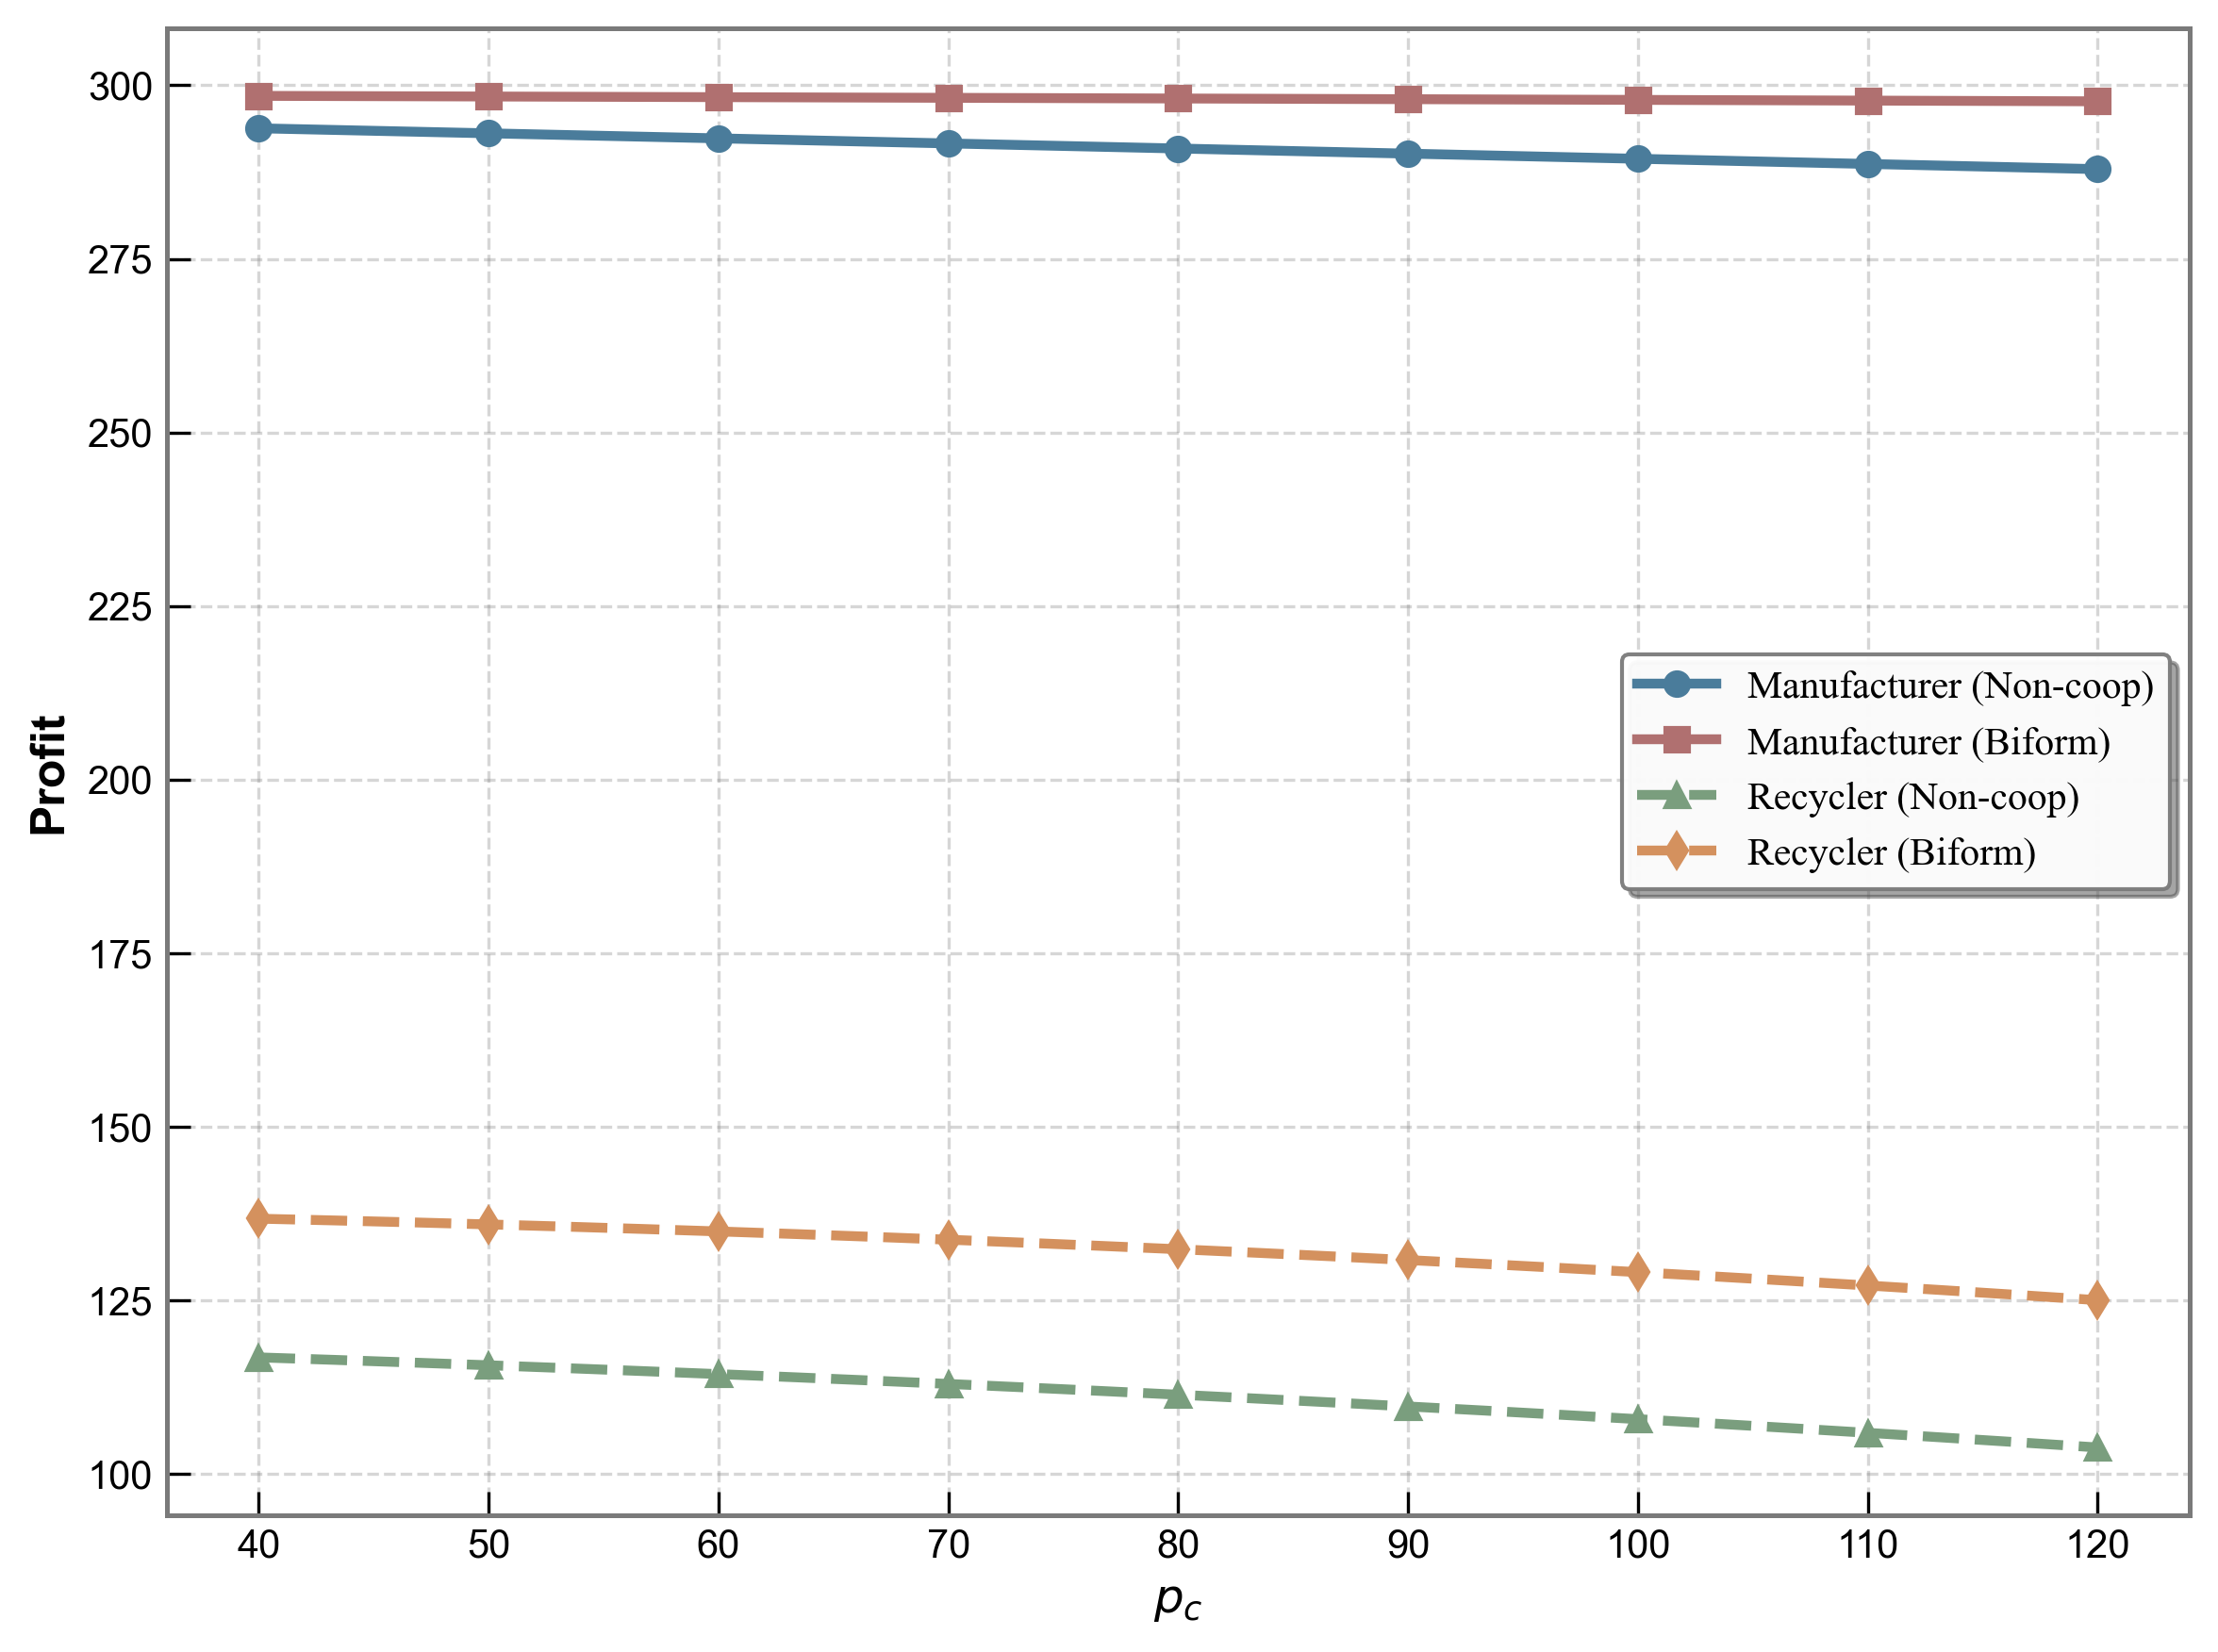
\includegraphics[width=0.45\textwidth]{fig1_profit_vs_pc.pdf}\label{fig:profit_vs_pc}}
\hfil
\subfloat[$\beta$]{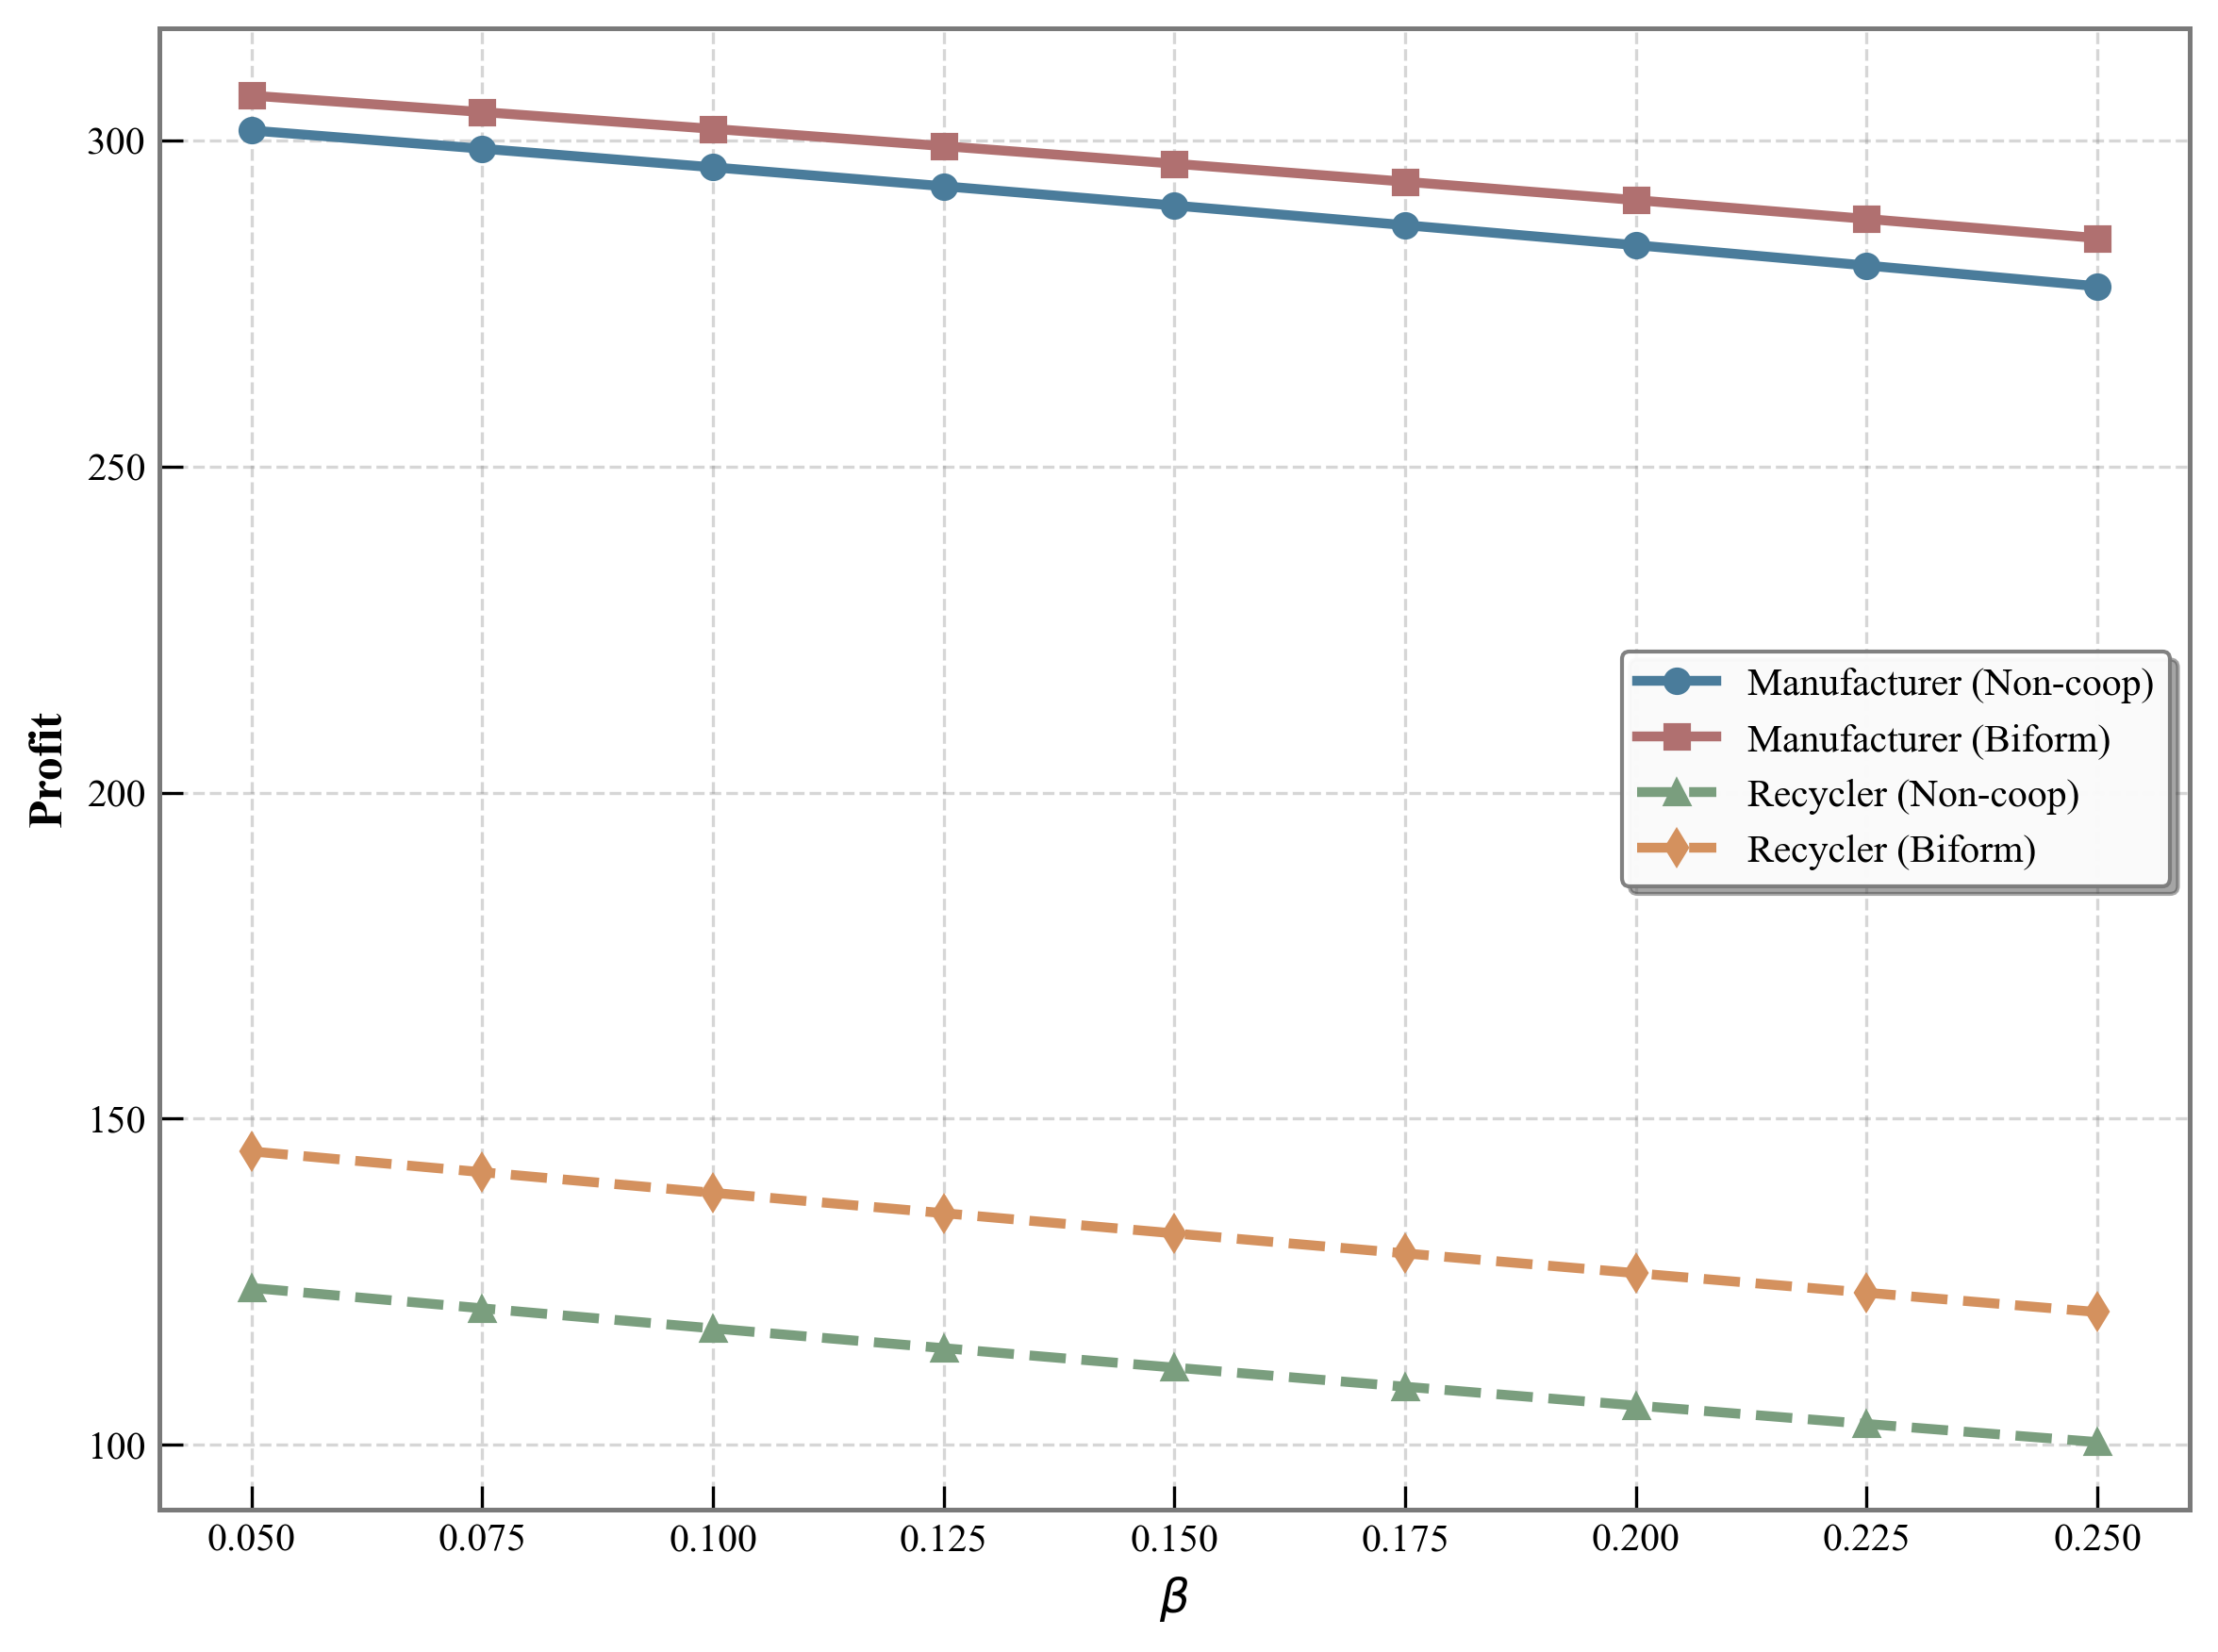
\includegraphics[width=0.45\textwidth]{fig2_profit_vs_beta.pdf}\label{fig:profit_vs_beta}}
\vfil
\subfloat[$\ln(c)$]{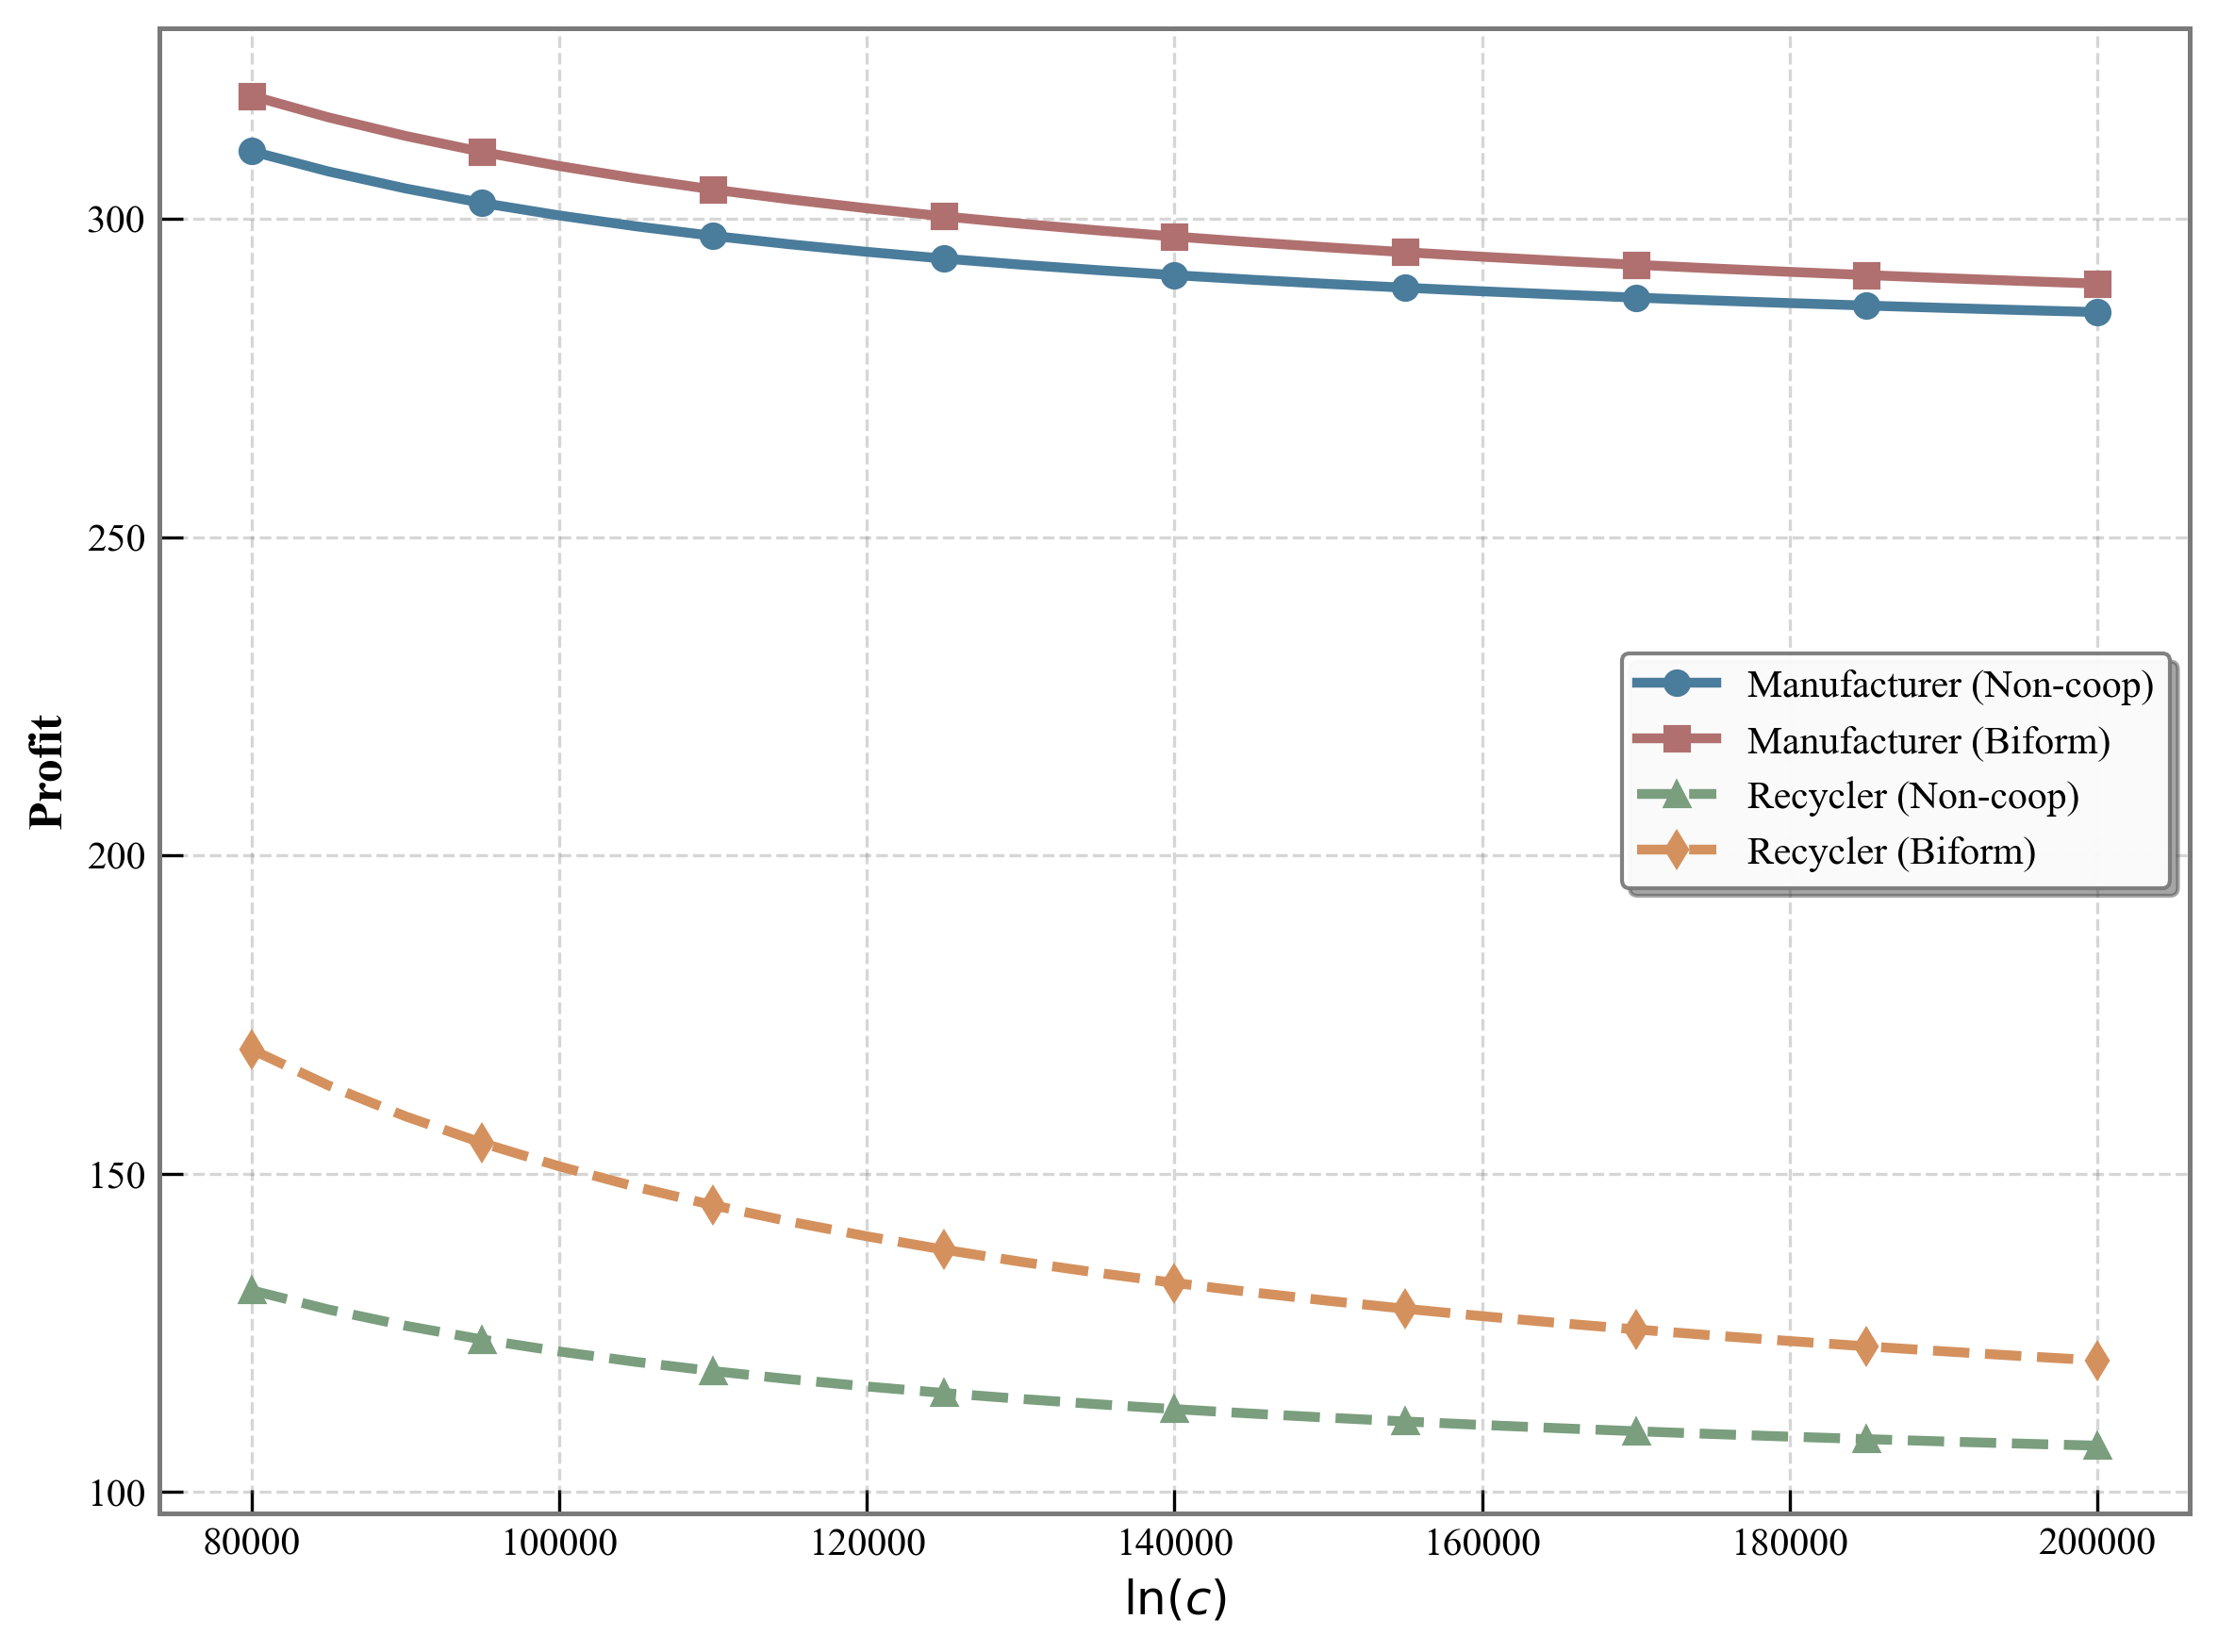
\includegraphics[width=0.45\textwidth]{fig3_profit_vs_c.pdf}\label{fig:profit_vs_c}}
\captionsetup{font=normalsize}
\caption{Profit comparison: Non-cooperative (baseline) vs Biform (cooperative) game}
\label{fig:profit_comparison}
\end{figure}

Fig. \ref{fig:profit_vs_beta} demonstrates the impact of competition intensity ($\beta$) on profits. As competition intensifies, both firms experience declining profits in both game frameworks. This pattern reflects the classic ``prisoner's dilemma'' in price competition: intensified competition compresses profit margins and forces firms to reduce collection efforts. Notably, the biform game consistently outperforms the non-cooperative baseline across all competition levels. The cooperative mechanism effectively alleviates destructive competition by aligning incentives: the manufacturer benefits from the recycler's technology improvements and thus has less incentive to engage in aggressive price cutting. The Shapley value allocation ensures that the cooperative surplus is fairly distributed, creating a win-win outcome that sustains the partnership even under fierce market competition.

Fig. \ref{fig:profit_vs_c} reveals the impact of the cost coefficient ($c$) on profits. As $c$ increases (representing higher technology investment costs), profits decline in both frameworks. The non-cooperative baseline is more sensitive to $c$ because the recycler bears the full investment burden. In contrast, the biform game's cost-sharing mechanism ($n^{C*}$), distributes the financial pressure, making profits less vulnerable to cost shocks. This finding highlights the importance of cooperative investment in promoting technology upgrading: under high investment cost environments, firms should prioritize strategic partnerships over independent R\&D to share risks and capture synergies.

Overall, the numerical results strongly support Propositions 5--8 in Section 4. The biform game achieves higher profits for both participants through the investment cost-sharing mechanism, demonstrating its effectiveness in coordinating the waste concrete recycling supply chain.

\subsubsection{Parameter Sensitivity Analysis}
\label{sec:sensitivity}

\noindent\textbf{(1) Impact of price sensitivity coefficient ($\alpha$) on recycling strategies.}
\label{sec:alpha_impact}

Figure 3 illustrates the impact of the price sensitivity coefficient ($\alpha$) on equilibrium outcomes. As $\alpha$ increases, waste generators become more responsive to changes in collection prices. The manufacturer's collection price ($p_M^*$) exhibits a monotonic upward trend, whereas the recycler's collection price ($p_R^*$) experiences a slight initial increase followed by a steady decline. The manufacturer consistently maintains a higher collection price compared to the recycler. This divergence stems from the inherent resource asymmetry between the two entities. The manufacturer capitalizes on its reverse logistics cost advantage to stimulate supply by raising prices. Conversely, the recycler, constrained by higher dedicated transportation costs and carbon emission liabilities under the cap-and-trade mechanism, rationally scales back its pricing strategy to control operational risks in the front-end collection market.

Concurrently, the collection quantities for both participants ($q_M^*, q_R^*$) and the total system collection ($Q^*$) expand significantly with an increase in $\alpha$. The manufacturer absorbs the majority of the market increment due to its sustained pricing advantage. The recycler's collection quantity continues to grow despite its reduced collection price, which is primarily driven by the overall expansion of the market scale activated by the high price sensitivity.

In the cooperative stage, the system conversion rate ($k^*$) rises gradually, while the proportion of investment cost borne by the recycler ($n^*$) exhibits a distinct monotonic decrease. As the total volume of collected waste concrete expands, the marginal benefit of improving the recycled concrete aggregate (RCA) quality increases. To ensure sufficient processing capability and higher RCA value, the manufacturer utilizes the surplus generated from its expanded collection market to bear a progressively larger share of the technology research and equipment upgrade costs. This dynamic demonstrates how the cooperative investment mechanism addresses the funding constraints of the specialized processor.

The economic outcomes indicate that both the manufacturer's profit ($\Pi_M^*$) and the recycler's profit ($\Pi_R^*$ ) increase, reflecting a mutual improvement in financial performance. Notably, the recycler maintains a higher absolute profit level and a steeper growth trajectory compared to the manufacturer. Within the delegated treatment framework, the recycler processes the extensive volume collected bythe manufacturer, generating stable transfer revenue. Furthermore, by shifting a significant portion ofthe capital expenditure tothe manufacturer throughthe cost-sharing agreement, the recycler effectively leverages its specialized processing capacity to capture a larger portion ofthe cooperative surplus.

\noindent\textbf{(2) Impact of government subsidy ($s$) on recycling strategies.}
\label{sec:s_subsidy_impact}

Figure 4 demonstrates the influence of the government subsidy ($s$) on the equilibrium decisions. The subsidy represents direct financial support provided per unit of collected waste concrete.

As shown in Figures 4(a) and 4(b), both collection prices ($p_M^*, p_R^*$) and collection quantities ($q_M^*, q_R^*$) exhibit a significant positive correlation with the subsidy level. The injection of government funds directly expands the profit margin of the supply chain. In response, both the manufacturer and the recycler translate this policy dividend into higher front-end collection prices to secure more waste resources. The manufacturer leverages its reverse logistics cost advantage to maintain a higher collection price and capture a larger market share. The synchronized price increases drive a substantial expansion in the total system collection quantity ($Q^*$).

Figure 4(c) illustrates the dynamics of the cooperative technology investment. The system conversion rate ($k^*$) increases steadily with $s$, while the recycler's cost-sharing ratio ($n^*$) rises sharply at lower subsidy levels before gradually stabilizing. In a low-subsidy environment, the recycler faces high downside risks for capital-intensive equipment upgrades and relies heavily on the manufacturer's financial support. As the subsidy increases, the guaranteed per-unit revenue effectively mitigates these investment risks. Consequently, the recycler's willingness to invest increases, leading it to assume a greater proportion of the technological costs. This indicates that government subsidies not only stimulate front-end collection but also serve as a catalyst for back-end capability upgrades by altering the risk-return profile of the specialized processor.

The profit trajectories in Figure 4(d) indicate that both participants experience substantial financial growth, validating the effectiveness of the subsidy policy in promoting industry development. The recycler's profit ($\Pi_R^*$) accelerates faster and remains consistently higher than the manufacturer's profit ($\Pi_M^*$). Within the delegated treatment model, the subsidy amplifies the volume of waste concrete transferred from the manufacturer to the recycler. The recycler processes this expanded volume, thereby maximizing its capacity utilization and economies of scale. Through the cooperative bargaining mechanism, the recycler leverages its indispensable processing capability to capture a premium from the subsidy-induced market expansion.

\noindent\textbf{(3) Impact of potential recycled value ($\theta$) on recycling strategies.}

Figure 5 presents the effect of the potential recycled value ($\theta$) on the equilibrium decisions. The parameter $\theta$ represents the maximum unit value of high-quality recycled concrete aggregate in the downstream market.

As illustrated in Figures 5(a) and 5(b), both collection prices ($p_M^*, p_R^*$) and collection quantities ($q_M^*, q_R^*$) exhibit a convex upward trend as $\theta$ increases. A higher $\theta$ signifies greater market potential for the end product, which expands the overall profit margin of the reverse supply chain. To capitalize on this, both the manufacturer and the recycler elevate their collection prices to secure a larger volume of waste concrete. The manufacturer sustains a consistently higher collection price due to its lower transportation costs ($\mu_M < \mu_R$). However, the recycler demonstrates a steeper price growth trajectory at high $\theta$ levels. As the direct producer of the recycled aggregate, the recycler is highly sensitive to the appreciation of the end-product value, which strengthens its pricing capability and aggressive procurement strategy in the front-end collection market.

Figure 5(c) shows that both the system conversion rate ($k^*$) and the recycler's cost-sharing ratio ($n^*$) increase significantly with $\theta$. Since the actual extracted unit value is the product of the potential value and the conversion rate ($\theta \times k^*$), a higher $\theta$ substantially amplifies the marginal return on technological investments. Driven by this strong economic incentive, the recycler becomes more willing to assume a larger proportion of the equipment upgrade costs ($n^*$) to achieve a higher conversion rate, thereby maximizing the revenue generated from high-quality recycled products.

Regarding the economic performance shown in Figure 5(d), both participants experience profit growth as $\theta$ increases. The recycler's profit ($\Pi_R^*$) is substantially higher than the manufacturer's profit ($\Pi_M^*$) and grows at a much faster rate. In environments with low potential value, the manufacturer's reverse logistics advantage plays a primary role in securing baseline returns. Conversely, as the potential value of the recycled material scales up, the recycler's specialized processing capability becomes the primary driver of value creation. The profit allocation mechanism in the cooperative stage reflects this fundamental shift in value drivers. Because the recycler is directly responsible for realizing the high potential value of the aggregate through processing, the Shapley value allocation enables it to capture a disproportionately larger share of the expanded market surplus.


\noindent\textbf{(4) Impact of outsourcing fee ($w$) and operational cost ($m$) on recycling strategies.}

Figures 6 and 7 illustrate how heterogeneous cost parameters—the internal outsourcing fee ($w$) and the external operational cost ($m$)—affect equilibrium decisions. These parameters demonstrate distinct transmission mechanisms within the supply chain.

Figure 7 shows the impact of the recycler's operational cost ($m$). As $m$ increases, the recycler experiences a direct contraction in its internal processing margin. Consequently, the recycler lowers its front-end collection price ($p_R^*$), which leads to a severe decline in its collection quantity ($q_R^*$). In contrast, the manufacturer's collection quantity ($q_M^*$) remains remarkably stable. The profit dynamics in Figure 7(b) reflect this isolation. The recycler's profit ($\Pi_R^*$) drops significantly as it absorbs the external operational cost burden, while the manufacturer's profit ($\Pi_M^*$) remains largely unaffected. This indicates that the delegated treatment model effectively shields the manufacturer from fluctuations in back-end processing costs.

Figure 6 presents the effects of the outsourcing fee ($w$), which acts as the internal transfer price. An increase in $w$ directly raises the manufacturer's procurement cost. As a result, the manufacturer substantially reduces its collection price ($p_M^*$), causing a steep downward trend in its collection quantity ($q_M^*$). The recycler's collection metrics ($p_R^*, q_R^*$) also decline, but at a more moderate pace.

Regarding profits, Figure 6(b) reveals a monotonic decline for both the manufacturer ($\Pi_M^*$) and the recycler ($\Pi_R^*$). The manufacturer's profit decreases due to the direct compression of its unit margin. Notably, the recycler's profit also declines steadily. While a higher $w$ increases the recycler's unit revenue from outsourced processing, it simultaneously triggers a severe contraction in the manufacturer's collection volume ($q_M^*$). Because the recycler relies on the manufacturer's substantial collection volume to maintain system scale and capacity utilization, the negative volume effect outweighs the positive price effect. Therefore, excessive internal transfer pricing generates system-wide friction, ultimately harming the economic performance of both participants.

\noindent\textbf{(5) Impact of transportation cost differential ($\mu_R - \mu_M$) on recycling strategies.}

Figure 8 displays the effect of the transportation cost differential ($\mu_R - \mu_M$) on the equilibrium outcomes. This parameter represents the magnitude of the manufacturer's reverse logistics advantage relative to the recycler's dedicated transportation cost.

As the cost differential widens, the recycler's collection price ($p_R^*$) and collection quantity ($q_R^*$) decrease significantly. The increasing logistics burden forces the recycler to lower its front-end procurement pricing to maintain operational viability. Because of this contraction, the total system collection quantity ($Q^*$) exhibits a pronounced downward trend. Concurrently, the manufacturer's collection price ($p_M^*$) and quantity ($q_M^*$) remain highly stable. This indicates that the manufacturer's front-end collection strategy is largely insulated from the recycler's specific logistics disadvantages.

In the cooperative stage, the recycler's cost-sharing ratio ($n^*$) decreases monotonically, accompanied by a slight decline in the system conversion rate ($k^*$). The escalating transportation costs directly diminish the recycler's financial capacity, thereby reducing its ability to fund technology and equipment upgrades. Furthermore, the continuous contraction in the total system collection volume limits the available economies of scale. The reduced volume provides less economic justification for high-level technological investments, leading to the gradual suppression of the overall conversion rate.

The profit distribution in Figure 8(d) demonstrates that the recycler's profit ($\Pi_R^*$) drops sharply as the cost differential expands, while the manufacturer's profit ($\Pi_M^*$) maintains stability. The external logistics friction is predominantly absorbed by the recycler. The substantial decline in the recycler's profitability negatively impacts the total cooperative surplus. This confirms that excessive asymmetry in logistics capabilities restricts the overall economic performance and technological advancement of the waste concrete recycling supply chain.

\section{Conclusion and implications}
\subsection{Conclusions}
This study constructs a non-cooperative and cooperative game model for waste concrete recycling involving manufacturers and recyclers. It investigates the collection price competition, technology cooperation, and R\&D cost sharing issues in the process of waste concrete recycling, as well as analyzes the impacts of external factors on recycling strategies. The conclusions of this study are as follows:

First, the manufacturer and the recycler tend to form a cooperative alliance to conduct the collection and processing of waste concrete. Within the optimal strategy portfolio across various scenarios in the coopetition relationship, the manufacturer's optimal pricing and collection quantity consistently exceed those of the recycler; meanwhile, the specialized recycler is required to bear a higher proportion of the investment costs for technological upgrading. This arrangement can effectively enhance the conversion rate of waste concrete into recycled aggregate and achieve a ``win-win'' outcome for the profits of both the manufacturer and the recycler.

Second, external engineering and market parameters exert significant heterogeneous impacts on the equilibrium decisions and profit distribution landscape of the manufacturer and the recycler. The results indicate that: the enhancement of the government subsidy $s$, price sensitivity $\alpha$, and potential recycled value $\theta$ can all significantly increase both parties' collection pricing, collection quantities, waste concrete conversion rates, and their respective profits; in particular, an increase in the potential recycled value $\theta$ drives the recycler's profit growth rate to be significantly higher than that of the manufacturer. Although the intensification of competition leads both parties to raise collection prices, the overall collection scale, conversion rate, and profits of both parties significantly decline as a result. An increase in the processing cost $m$ primarily leads to a unilateral decline in the recycler's collection quantity and profit; conversely, an increase in the outsourcing fee $w$ suppresses the manufacturer's collection quantity and causes the recycler's profit to exhibit an inverted-U trajectory, initially rising and then falling. Furthermore, an increase in transportation costs exerts a suppressive effect on a firm's own collection strategy. High unilateral transportation costs not only trigger a precipitous drop in the affected firm's collection quantity and profit but also diminish the overall willingness to invest in technology, leaving the system's actual technology conversion rate at a depressed level.

\subsection{Theoretical implications}

% TODO: Write content here

\subsection{Practical implications}

% TODO: Write content here

\section{Limitations and future research directions}
There are certain limitations that highlight avenues for future research. First, this study primarily focuses on a basic dual-channel supply chain consisting of a single traditional manufacturer and a single specialized recycler. However, the actual waste concrete recycling ecosystem often involves more complex interactions among multiple stakeholders. Future research could expand the current modeling framework to incorporate multiple competing recyclers, third-party logistics providers, or explicitly consider the downstream demand market's acceptance of recycled materials, thereby more comprehensively revealing the operational mechanisms of a closed-loop supply chain network with multi-party participation.

Second, this research employs a static game framework to analyze the equilibrium decisions and profit distribution of supply chain members. Future research could integrate differential games or evolutionary game theory to explore the dynamic evolutionary trajectories of enterprises' technology R\&D investments over multiple periods, as well as the long-term stability conditions of the outsourcing cooperation.

\section*{Data availability statement}
% TODO: Write data availability statement here

\section*{Declaration of competing interest}
% TODO: Write declaration here

% ===== 参考文献 =====

\appendix

\appendix
\section{Proof of Proposition \ref{prop:baseline}}
\label{app:prop1}

We solve the non-cooperative game using backward induction.

\textbf{Step 1: Recycler's technology investment decision.} Given collection prices $(p_M, p_R)$, the recycler $R$ chooses $k$ to maximize $\Pi_R^N$ in Equation \eqref{eq:profit_RN}. Taking the first-order derivative with respect to $k$:
\begin{equation}
\frac{\partial \Pi_R^N}{\partial k} = \theta(\alpha p_R - \beta p_M) - ck = 0
\end{equation}
Solving for $k$, we obtain the optimal conversion rate:
\begin{equation}
k^N(p_M, p_R) = \frac{\theta(\alpha p_R - \beta p_M)}{c}
\tag{A1}
\end{equation}

Substituting (A1) into $\Pi_R^N$, the recycler's profit becomes:
\begin{equation}
\Pi_R^N =
\begin{aligned}
& (s - p_R - m - \mu_R)(\alpha p_R - \beta p_M) + (w - m)(\alpha p_M - \beta p_R) \\
& + \frac{\theta^2(\alpha p_R - \beta p_M)^2}{2c} - p_c\left[ e(\alpha - \beta)(p_M + p_R) - G \right]
\end{aligned}
\tag{A2}
\end{equation}

\textbf{Step 2: Price competition equilibrium.} Using the profit functions $\Pi_M^N$ and $\Pi_R^N$, we derive the reaction functions by taking first-order partial derivatives with respect to $p_M$ and $p_R$, respectively, and setting them equal to zero:
\begin{equation}
\frac{\partial \Pi_M^N}{\partial p_M} = (\theta k - p_M - w - \mu_M + s)\alpha - (\alpha p_M - \beta p_R) = 0
\tag{A3}
\end{equation}
\begin{equation}
\frac{\partial \Pi_R^N}{\partial p_R} =
\begin{aligned}
& (s - p_R - m - \mu_R)\alpha + \theta\alpha k^N - \alpha p_R + (w - m)(-\beta) \\
& - p_c e (\alpha - \beta) = 0
\end{aligned}
\tag{A4}
\end{equation}

Substituting $k^N$ from (A1) into (A4), and solving the system of (A3)-(A4) simultaneously, we obtain the equilibrium collection prices $p_M^{N*}$ and $p_R^{N*}$, which are given by Equations \eqref{eq:p_MN_star} and \eqref{eq:p_RN_star} in Proposition \ref{prop:baseline}. Substituting these equilibrium prices back into (A1) yields $k^{N*}$ in Equation \eqref{eq:k_N_star}. The equilibrium collection quantities and profits follow directly from substituting the equilibrium values into the profit functions. This completes the proof. \hfill $\square$

\section{Proof of Proposition \ref{prop:characteristic}}
\label{app:prop2}

We compute the characteristic functions for each coalition using the maximin principle.

\textbf{(1) Coalition $\{M\}$.} The characteristic function is:
\begin{equation}
V_{p_M,p_R}(\{M\}) = \max_{n \in [0,1]} \min_{k \in [0,1]} \{\Pi_M\}
\end{equation}
Since $\Pi_M = (\theta k + s - p_M - w - \mu_M)(\alpha p_M - \beta p_R) - (1 - n)\frac{ck^2}{2}$ and $(\alpha p_M - \beta p_R) \geq 0$, for any given $n$, the term is minimized when $k = 0$. Maximizing over $n \in [0,1]$ yields $n^* = 1$, which eliminates the investment cost term. Therefore:
\begin{equation}
V_{p_M,p_R}(\{M\}) = (s - p_M - w - \mu_M)(\alpha p_M - \beta p_R)
\tag{B1}
\end{equation}

\textbf{(2) Coalition $\{R\}$.} The characteristic function is:
\begin{equation}
V_{p_M,p_R}(\{R\}) = \max_{k \in [0,1]} \{\Pi_R\}
\end{equation}
Setting $n = 1$ (the recycler bears all costs) and taking the first-order derivative with respect to $k$:
\begin{equation}
\frac{\partial \Pi_R}{\partial k} = \theta(\alpha p_R - \beta p_M) - ck = 0
\end{equation}
Solving yields $k^* = \frac{\theta(\alpha p_R - \beta p_M)}{c}$. Substituting into $\Pi_R$:
\begin{equation}
V_{p_M,p_R}(\{R\}) =
\begin{aligned}
& \left(s - p_R - m - \mu_R\right)(\alpha p_R - \beta p_M) + (w - m)(\alpha p_M - \beta p_R) \\
& + \frac{\theta^2(\alpha p_R - \beta p_M)^2}{2c} - p_c\left[ e(\alpha-\beta)(p_M+p_R)-G\right]
\end{aligned}
\tag{B2}
\end{equation}

\textbf{(3) Grand coalition $\{M,R\}$.} The characteristic function is:
\begin{equation}
V_{p_M,p_R}(\{M,R\}) = \max_{k \in [0,1]} \{\Pi_M + \Pi_R\}
\end{equation}
Taking the first-order derivative:
\begin{equation}
\frac{\partial (\Pi_M + \Pi_R)}{\partial k} = \theta(\alpha p_M - \beta p_R) + \theta(\alpha p_R - \beta p_M) - ck = 0
\end{equation}
Solving yields $k^* = \frac{\theta(\alpha - \beta)(p_M + p_R)}{c}$. Substituting:
\begin{equation}
V_{p_M,p_R}(\{M,R\}) =
\begin{aligned}
& (s - p_M - m - \mu_M)(\alpha p_M - \beta p_R) + (s - p_R - m - \mu_R)(\alpha p_R - \beta p_M) \\
& + \frac{\theta^2(\alpha - \beta)^2(p_M + p_R)^2}{2c} - p_c\left[ e(\alpha-\beta)(p_M+p_R)-G\right]
\end{aligned}
\tag{B3}
\end{equation}

Equations (B1)-(B3) correspond to the characteristic functions stated in Proposition \ref{prop:characteristic}. This completes the proof. \hfill $\square$

\section{Proof of Proposition \ref{prop:convexity}}
\label{app:prop3}

From Proposition \ref{prop:characteristic}, we compute the surplus from forming the grand coalition:
\begin{equation}
\begin{aligned}
& V_{p_M,p_R}(\{M,R\}) - V_{p_M,p_R}(\{M\}) - V_{p_M,p_R}(\{R\}) \\
&= \frac{\theta^2(\alpha - \beta)^2(p_M + p_R)^2}{2c} - \frac{\theta^2(\alpha p_R - \beta p_M)^2}{2c} \\
&= \frac{\theta^2}{2c}(\alpha p_M - \beta p_R)\big[(\alpha p_M - \beta p_R) + 2(\alpha p_R - \beta p_M)\big]
\end{aligned}
\tag{C1}
\end{equation}

Since $\alpha > \beta > 0$ by assumption, we have $(\alpha p_M - \beta p_R) \geq 0$ and $(\alpha p_R - \beta p_M) \geq 0$. Additionally, $\theta > 0$ and $c > 0$. Therefore, the right-hand side of (C1) is always non-negative. Hence:
\begin{equation}
V_{p_M,p_R}(\{M,R\}) \geq V_{p_M,p_R}(\{M\}) + V_{p_M,p_R}(\{R\})
\end{equation}
which establishes superadditivity. Furthermore, the marginal contribution of each player increases with the size of the coalition, satisfying the convexity condition. Consequently, the Shapley value allocation belongs to the core of the cooperative game. This completes the proof. \hfill $\square$

\section{Proof of Proposition \ref{prop:biform}}
\label{app:prop4}

Having established the characteristic functions and Shapley value allocations $\varphi_M(p_M, p_R)$ and $\varphi_R(p_M, p_R)$ in Section \ref{sec:biform_model}, we now solve the non-cooperative price competition stage.

\textbf{Step 1: Concavity verification.} Taking second-order partial derivatives of $\varphi_M$ and $\varphi_R$ with respect to their respective prices:
\begin{equation}
\frac{\partial^2 \varphi_M}{\partial p_M^2} = \frac{\theta^2(\alpha^2 - 2\alpha\beta)}{2c}
\quad \text{and} \quad
\frac{\partial^2 \varphi_R}{\partial p_R^2} = \frac{\theta^2(2\alpha^2 - 2\alpha\beta + \beta^2)}{2c}
\end{equation}
When $\alpha > 2\beta > 0$, both second-order derivatives are negative, confirming strict concavity of the profit allocation functions.

\textbf{Step 2: First-order conditions.} Setting the first-order partial derivatives to zero:
\begin{equation}
\begin{cases}
\frac{\partial \varphi_M}{\partial p_M} = [\theta^2(\alpha^2 - 2\alpha\beta) - 4c\alpha]p_M + [\theta^2(\alpha^2 - \alpha\beta + \beta^2) + 2c\beta]p_R + 2c\alpha(s - w - \mu_M) = 0 \\
\frac{\partial \varphi_R}{\partial p_R} = [\theta^2(\alpha^2 - 3\alpha\beta + \beta^2) + 2c\beta]p_M + [\theta^2(2\alpha^2 - 2\alpha\beta + \beta^2) - 4c\alpha]p_R + 2c[\alpha(s - m - \mu_R) - \beta(w - m)] - 2c p_c e (\alpha - \beta) = 0
\end{cases}
\tag{D1}
\end{equation}

\textbf{Step 3: Solving the reaction functions.} Solving the linear system (D1) yields the equilibrium collection prices $p_M^{C*}$ and $p_R^{C*}$, which are given by Equations (27) and (28) in Proposition \ref{prop:biform}.

\textbf{Step 4: Optimal conversion rate and cost-sharing proportion.} Substituting $p_M^{C*}$ and $p_R^{C*}$ into the grand coalition's optimal $k$:
\begin{equation}
k^{C*} = \frac{\theta(\alpha - \beta)(p_M^{C*} + p_R^{C*})}{c}
\end{equation}
The optimal cost-sharing proportion $n^{C*}$ is derived by equating the marginal contributions and solving for $n$, yielding the expression in Proposition \ref{prop:biform}.

The equilibrium Shapley value allocations $\varphi_M^{C*}$ and $\varphi_R^{C*}$ follow directly from substituting the equilibrium prices into the Shapley value formulas. This completes the proof. \hfill $\square$

\bibliographystyle{elsarticle-harv}
\bibliography{zz05}

% ===== 表格模板（复制使用） =====

% \begin{table}[!htbp]
% \centering
% \captionsetup{font=normalsize, labelsep=period}
% \setlength{\abovecaptionskip}{5pt}
% \setlength{\belowcaptionskip}{0pt}
% \caption{Table title here}
% \label{tab:label_name}
% \small
% \begin{threeparttable}
% \begin{tabular*}{0.9\textwidth}{@{\extracolsep{\fill}}lccccccc}
% \toprule
% \textbf{Column 1} & \textbf{Column 2} & \textbf{Column 3} & \textbf{Column 4} \\
% \midrule
% \textit{Row 1} & Data & Data & Data \\
% \textit{Row 2} & Data & Data & Data \\
% \textit{Row 3} & Data & Data & Data \\
% \bottomrule
% \end{tabular*}
% \begin{tablenotes}[flushleft]
% \small\linespread{1}\selectfont
% \item \textit{Note}: Table notes here.
% \end{tablenotes}
% \end{threeparttable}
% \end{table}
% \vspace{-15pt}

\end{document}
